\ifcase0  % choose 0=slides, 1=article, 2=refart
	 \documentclass[ignorenonframetext,12pt]{beamer}
	 \geometry{paper=a6paper,landscape}
\or\documentclass[a4paper,11pt]{article}
	 \usepackage{url,beamerarticle}
\or\documentclass[a4paper,11pt]{refart}
	 \let\example\relax
	 \usepackage{url,beamerarticle}
\fi

\ifcase0  % choose a theme like these
	 \usetheme{Montpellier}% I recommend
\or\usetheme{Singapore}
\or\usetheme{Szeged}
\or\usetheme{Boadilla}
\or\usetheme{Pittsburgh}
\or\usetheme{Madrid}
\or\usetheme{Warsaw} % common choice, but often poor
\fi

\usepackage{graphicx,pgfplots,parskip}
\graphicspath{{media/}}



\title{QUBIC mettings} 
\author{Horacio Arnaldi\\
Laboratorio Detecci\'on de Part\'iculas y Radiaci\'on\\
CAB-IB}
\date{August 1, 2019}

\begin{document}

\begin{frame}
				\maketitle
\end{frame}

\begin{abstract}
				This abstract, being outside the frame environment, does not appear in the presentation.  Your outline will be the basis for a couple of sentences of talk for each of the following questions:
				\begin{itemize}
								\item What was done?
								\item Why do it?
								\item What were the results?
								\item What do the results mean in theory and/or practise?
								\item What is the reader's benefit?
								\item How can the readers use this information for themselves? 
				\end{itemize}
\end{abstract}

\begin{frame}{Outline}
				\tableofcontents
\end{frame}

\section{Readout design and development}
\begin{frame}{Readout design and development}

				{\color[rgb]{0.8,.4,.5} ``The readout electronics have the general task of performing multiple
				real-time complex microwave transmission measurements, in order to
				monitor the instantaneous resonance frequency and dissipation of the
				superconducting microresonators that serve as mm/submm photon
				detectors''.}

				Noise will be dominated by cryogenic HEMT amplifier, which has noise
				temperature around 2 to 5 K. Besides the HEMT, ADC chip will be the next
				limiting factor for the noise performance of the readout. 

				Based on the physical frequency spacing of all the resonators, the
				sampling rate are chosen to match the resonator bandwidth. Sampling rate
				of proposed readout system can be flexible.
				Right now it is up to 550 MHz which is the limit of ADC chip.

				\emph{\textbf{An open-source readout for MKIDs}}, Proc. SPIE Astron. Telesc.
				Instrum., doi:10.1117/12.856832
\end{frame}
\begin{frame}{Readout design and development}

				MKIDs $\to$ 

				The obvious advantage of MKIDs over competing cryogenic technologies
				like TESs is the elimination of the cryogenic electronics required for multiplexing

				\emph{\textbf{A readout for large arrays of microwave kinetic inductance
				detectors}}, Rev. Sci. Instrum., doi:10.1063/1.3700812
\end{frame}
\begin{frame}{Channelizer Tx}
				%\begin{columns}
				%				\begin{column}{0.65\textwidth}
				\begin{center}
								\only<1>{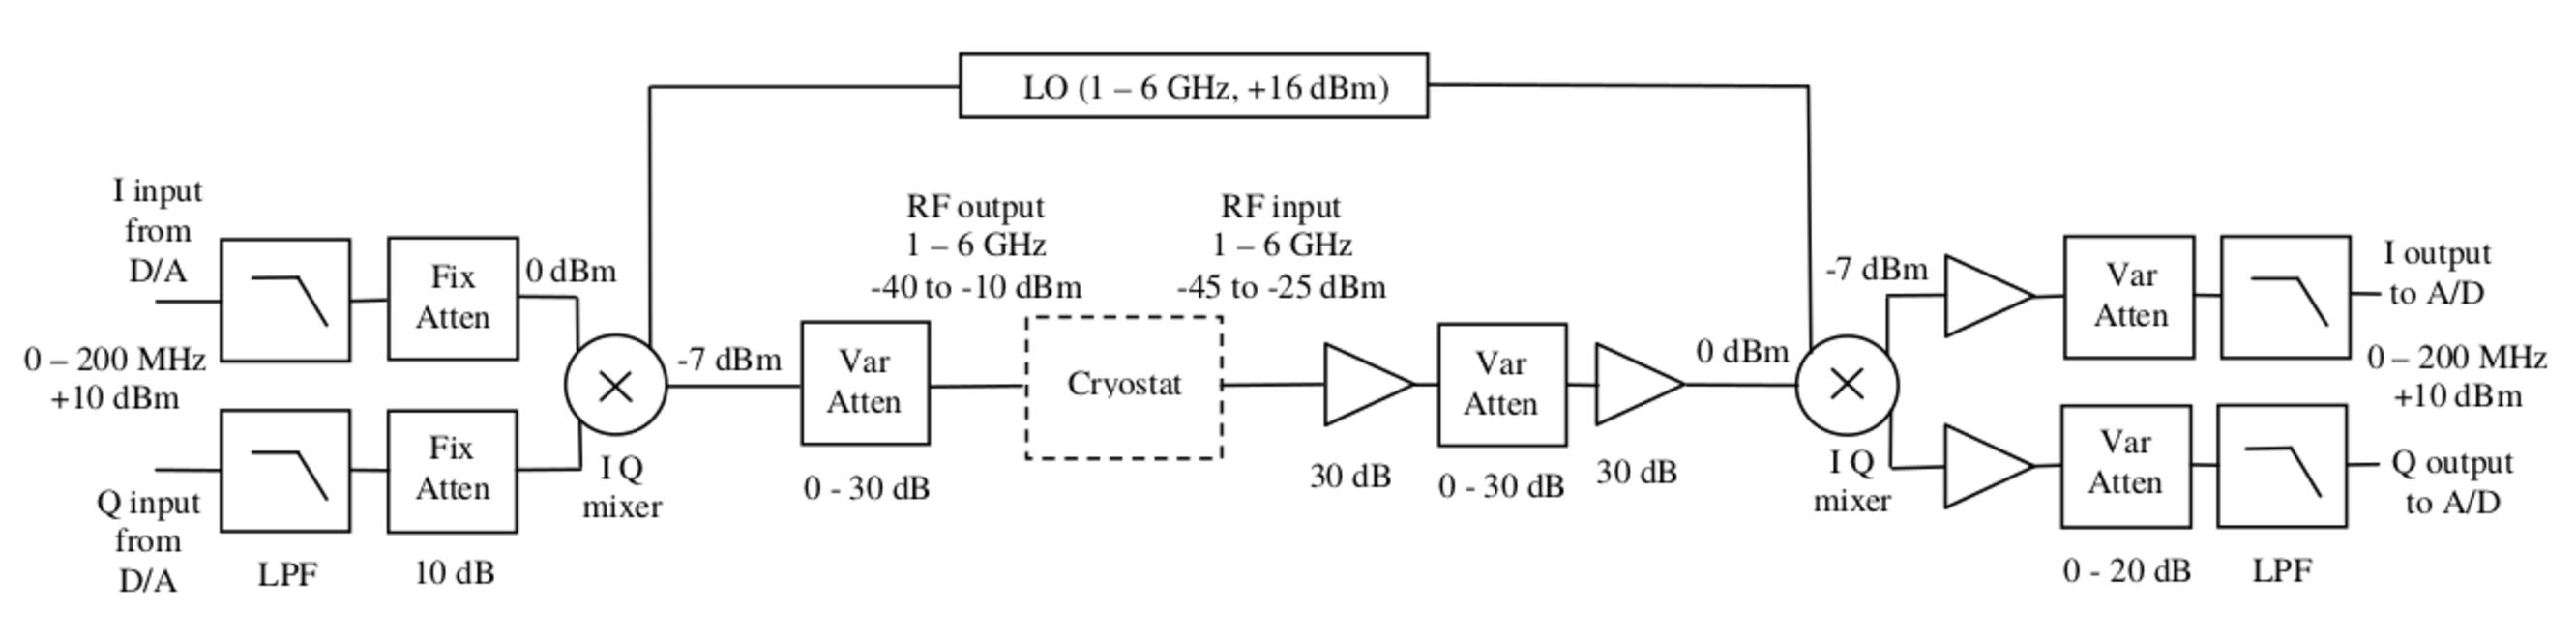
\includegraphics[width=\textwidth]{if_electronic_schematic}}
				\end{center}
				%				\end{column}
				%				\begin{column}{0.65\textwidth}
								\begin{center}
												\only<2>{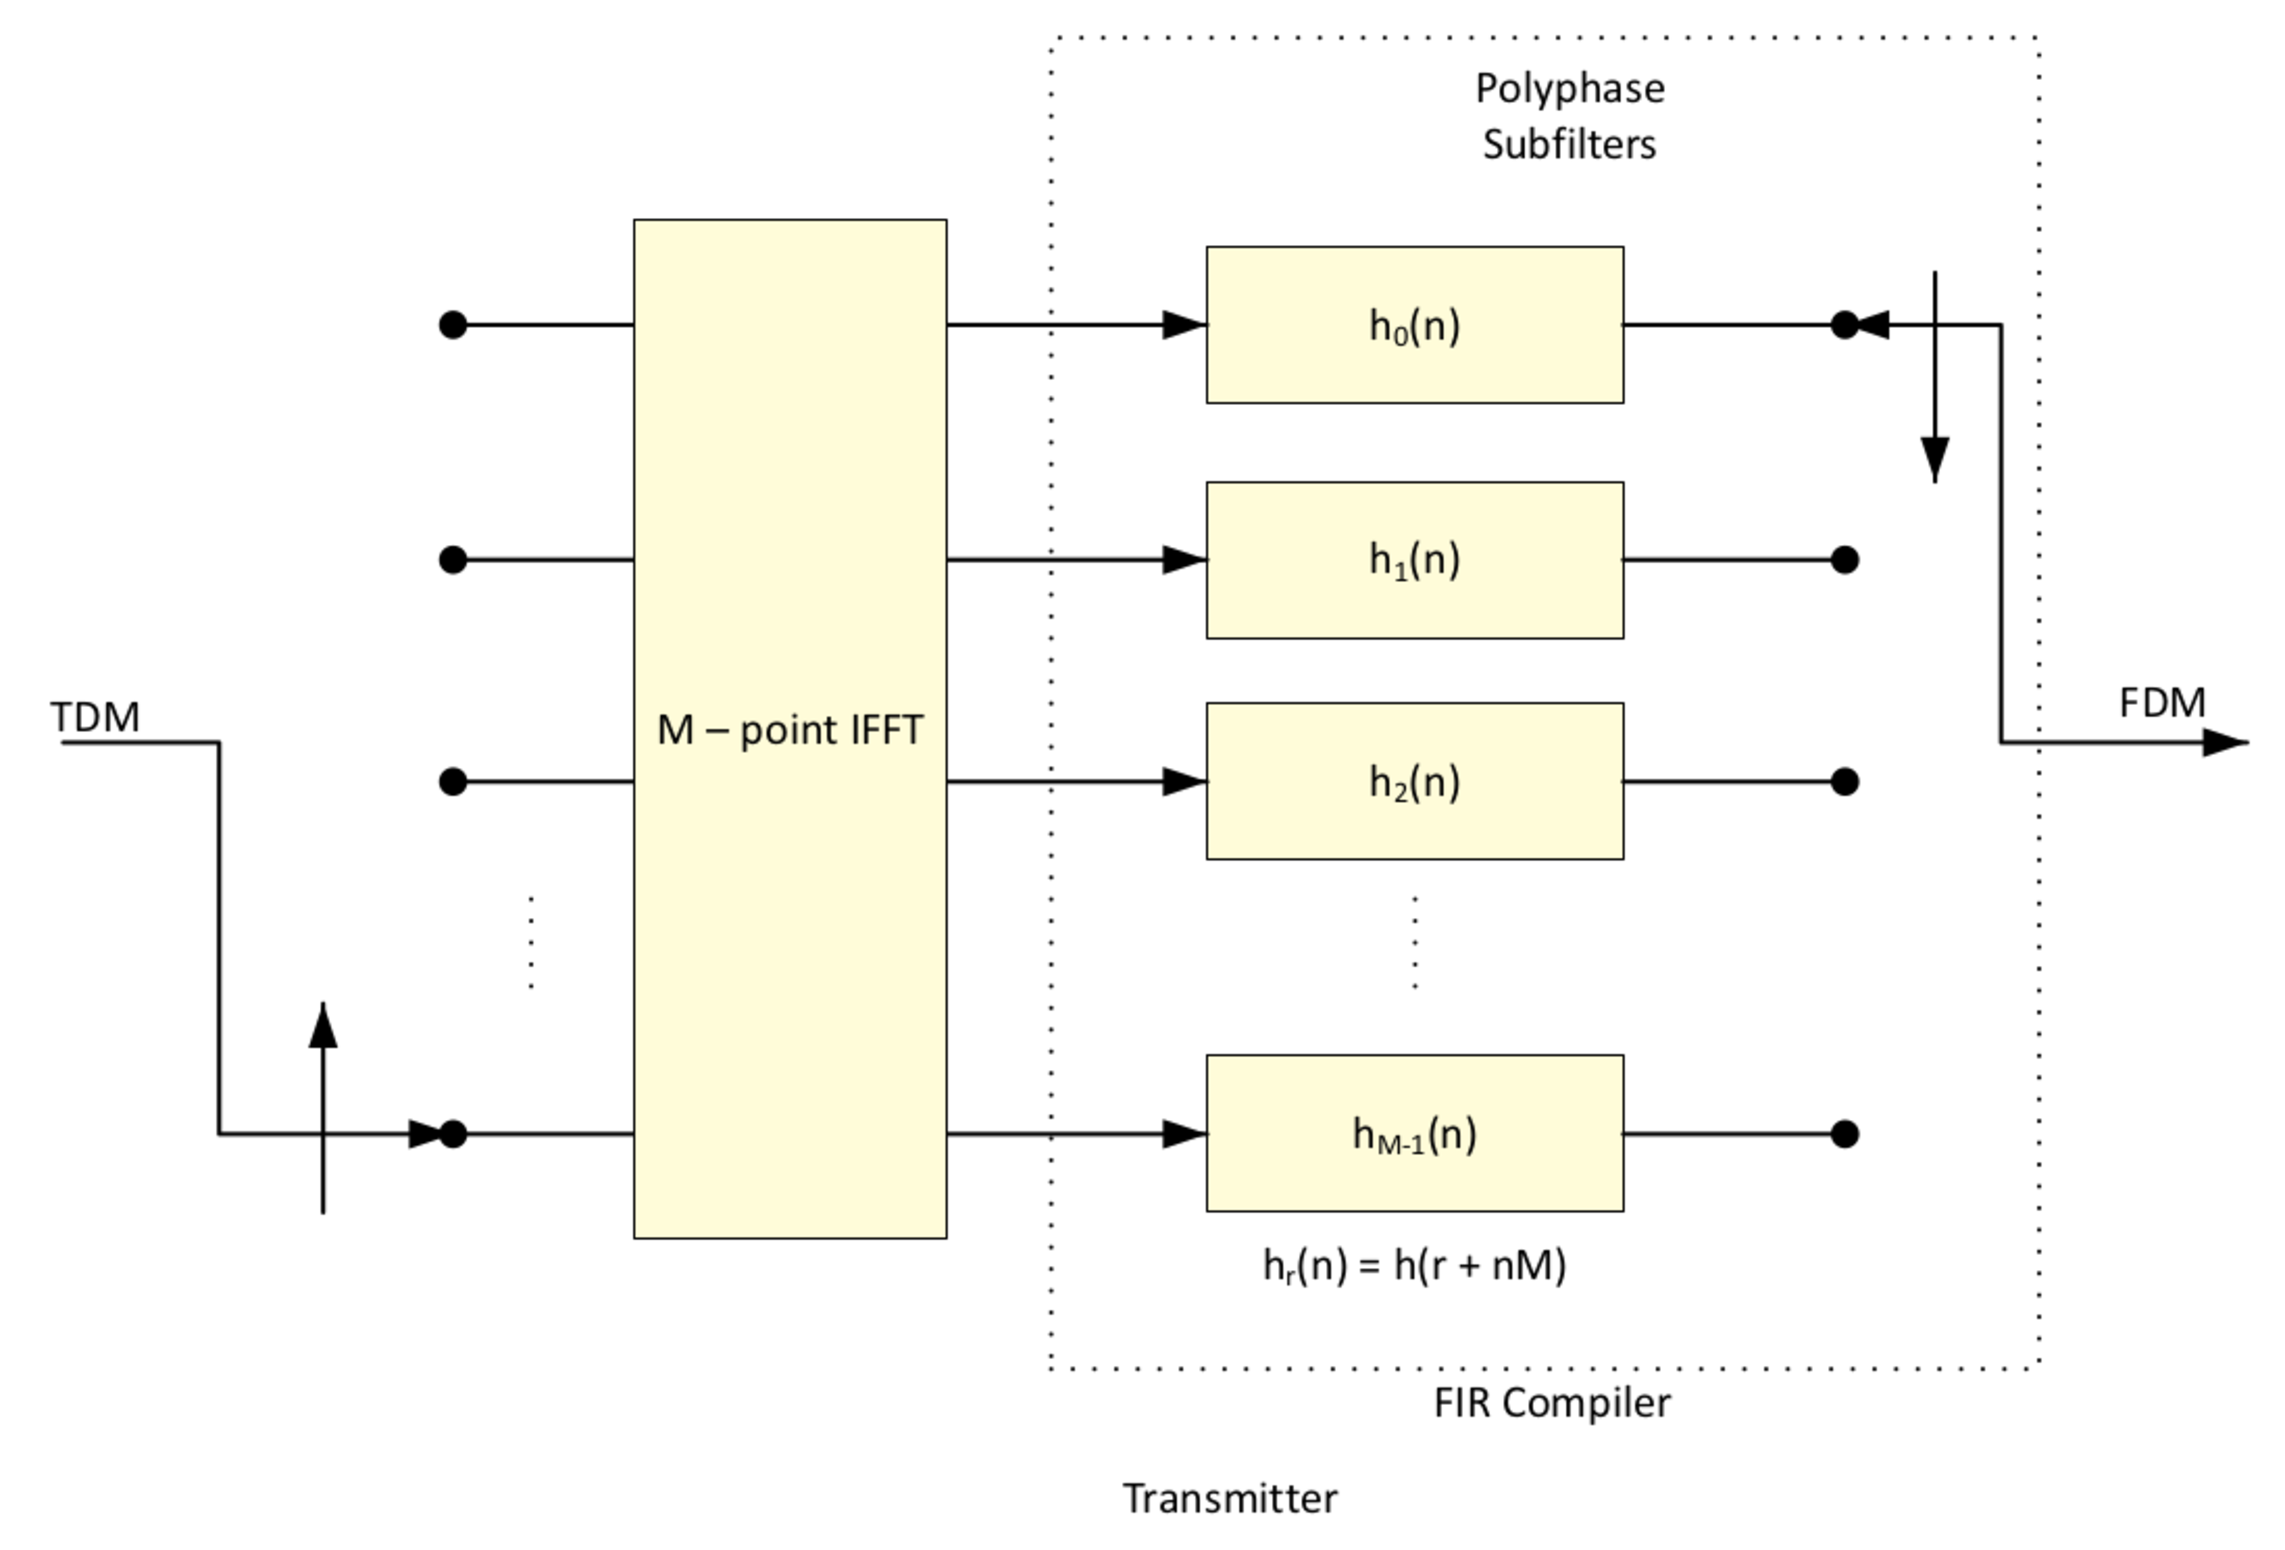
\includegraphics[width=0.8\textwidth]{Tx_channelizer_con_IFFT}}
								\end{center}
								%				\end{column}
								%\end{columns}
\end{frame}

\begin{frame}{Design requirements}
				\begin{itemize}
								\item The readout must not introduce significant noise above the
												system noise floor set by the \textbf{cryogenic
												amplifier}
												with a noise temperature of $\sim 4\,\text{K}$.
								\item The entire readout system must be capable of
												reading out at least 512 resonators in $\sim
												1\,\text{GHz}$ of bandwidth ({\color{red} to be
												confirmed}).
								\item Crosstalk between channels greater than $250\,\text{kHz}$
												apart should be less than 1\%.
								\item Intrinsic energy resolution $R \sim
												20-150$\footnote{Rev.Sci.Instr. 83, 044702 (2012)}
								\item 
								\item 
				\end{itemize}
\end{frame}

\section{MKIDs}
\begin{frame}{MKIDs}
				\begin{columns}
								\begin{column}{0.49\textwidth}
												\footnotesize{The KID detection mechanism is manifested
												by a temporal change in the surface kinetic inductance
												of a superconductor when a photon of energy $h\nu \geq
												2 \Delta(T)$ is absorbed, where $\Delta(T)$ is the
												superconducting gap parameter. High energy photons break
												Cooper pairs. These recombine in a characteristic time,
												of the order $10-500\,\mu\text{s}$,
												{\color{red}producing pulse-like changes in the surface
												impedance}. As the impedance of a superconductor is
												mostly inductive, especially for $T << T_c$, the
												superconductor can be engineered as the inductive
												element in a RLC-like resonant circuit. {\color{blue}The
												quality factor of the resonant circuit determines both the
												sensitivity and speed of the device}.}

								\end{column}
								\begin{column}{0.49\textwidth}
								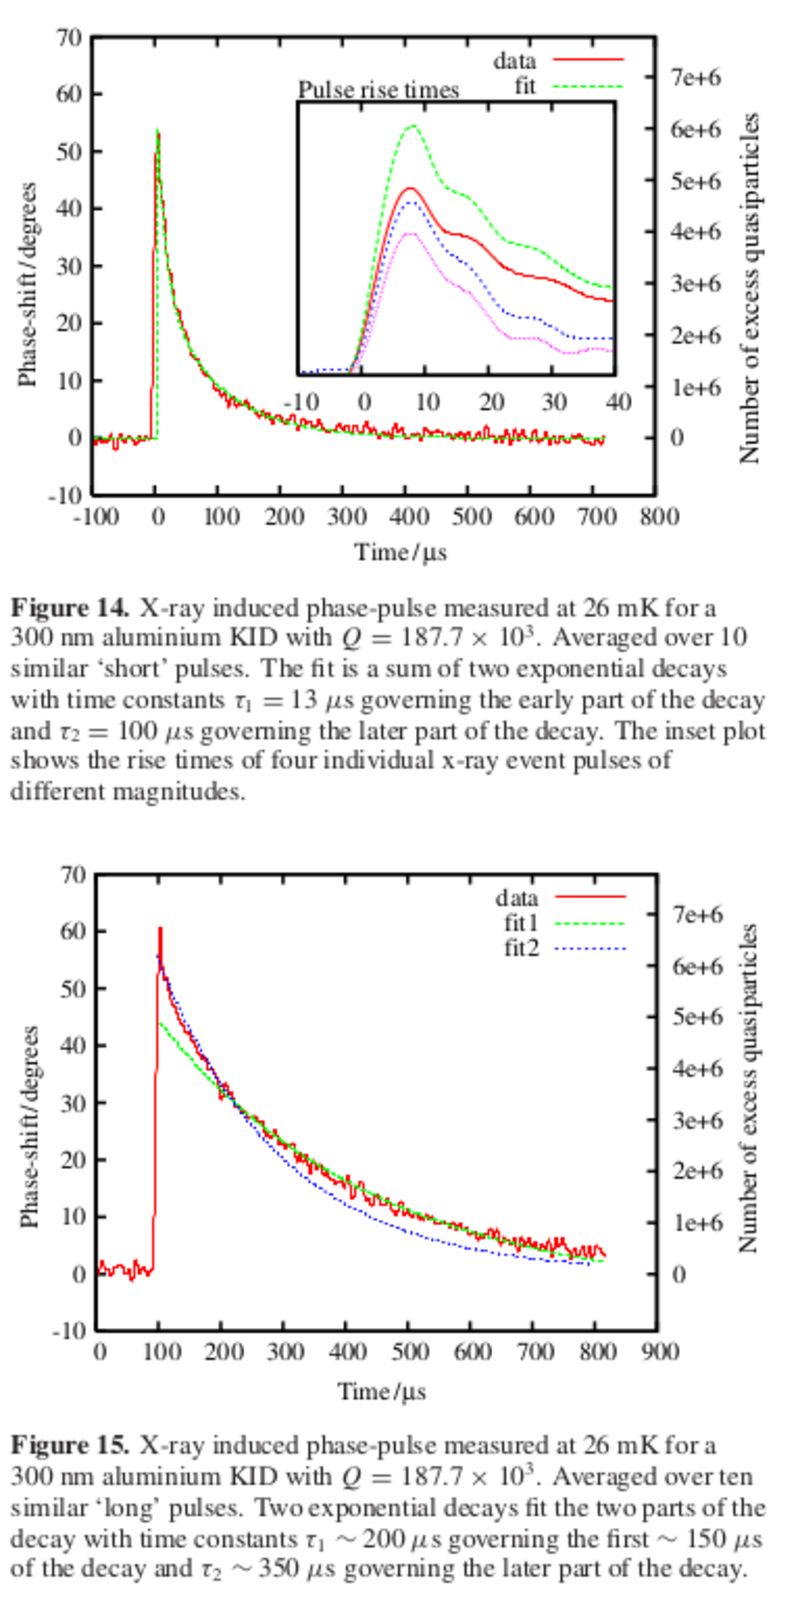
\includegraphics[width=0.62\textwidth]{pulso_respuesta_mkid}
								\end{column}
				\end{columns}
\end{frame}

\begin{frame}{MKIDs}
				\begin{exampleblock}{}
								Works on the principle that incident photons change the surface
								impedance of a superconductor through the \textit{kinetic
								inductance effect}
				\end{exampleblock}
												\begin{equation}
																R = \frac{1}{2.355}\sqrt{\frac{\eta h \nu}{F
																\Delta}}
												\end{equation}
				where $\eta = 0.57$ is the efficiency of creating quasiparticles, $h\nu$
				is the energy of the incident photon, $\Delta = 1.72k_BT_c$ is the gap
				energy of the superconducting absorber, and $F \approx 0.2$ is the Fano
				factor. This works out to $R=150$ at 5\,eV for an operating temperature
				of 100\,mK. An operating temperature of 15\,mK could allow a theoretical
				maximum energy resolution of R=400 at 5\,eV, although it is likely other
				noise sources, like two level system noise, will become more important
				as future development increases the energy resolution.

\end{frame}
\begin{frame}{MKIDs}
				\begin{exampleblock}{}
								Works on the principle that incident photons change the surface
								impedance of a superconductor through the \textit{kinetic
								inductance effect}
				\end{exampleblock}
				\begin{itemize}
								\item Resonance  $1-10\,\text{GHz}$ 
								\item $Q \sim 10^5$
								\item $T_{op} < 300\,\text{mK}$
								\item Intrinsic energy resolution $R = \frac{E}{\Delta E} \sim
												20-150$\footnote{Rev.Sci.Instr. 83, 044702 (2012)}
								\item The resonators are designed to be separated by 2 MHz
												within a $4-5\,\text{GHz}$ band.
								\item 
												\begin{equation}
																R = \frac{1}{2.355}\sqrt{\frac{\eta h \nu}{F
																\Delta}}
												\end{equation}
				\end{itemize}

				\textbf{arXiv:1310.5891v2 (2013)}
\end{frame}

\begin{frame}{The cryogenic amplifier}
				\begin{itemize}
								\item The double sideband (DSB) phase noise of the HEMT
												amplifier is given by the simple expression, 
												{\color{red}
												\begin{equation}
																\frac{k_B T_n}{P}
												\end{equation}} 
												where $T_n$ is noise temperature of the
												amplifier, and $P$ is the power on the input. The
												readout power for each MKID should be $-100 \pm
												15\,\text{dBm}$ ({\color{red} to be confirmed}). For
												$-85\,\text{dBm}$ readout power, off resonance, and $T_n
												= 6\,\text{K}$, we expect $-106\,\text{dBc/Hz}$ for the
												HEMT phase noise. Ideally, the readout electronics will
												contribute noise well below this value.\footnote{Rev.Sci.Instr. 83, 044702 (2012)}
				\end{itemize}
\end{frame}

\begin{frame}{The cryogenic amplifier}
				Rev.Sci.Instr. 83, 044702 (2012)
				\begin{columns}
								\begin{column}{0.45\textwidth}
												\begin{itemize}
																\item \footnotesize{Given an ADC's voltage noise
																				specification, the number of channels
																				$n$ an ADC can read out at a given power
																				without adding to the HEMT noise can be
																				calculated.}
																\item The contours of Fig. 3 are calculated by
																				scaling the HEMT noise with a
																				channel-dependent factor giving, $k_B
																				T_n /(p_\text{max}^2 P)$.
																\item $p_\text{max} \propto
																				n^{1/2}\,\text{for}\,n >> 1$
																\item Random phase per tone assumed
												\end{itemize}
								\end{column}
								\begin{column}{0.45\textwidth}
								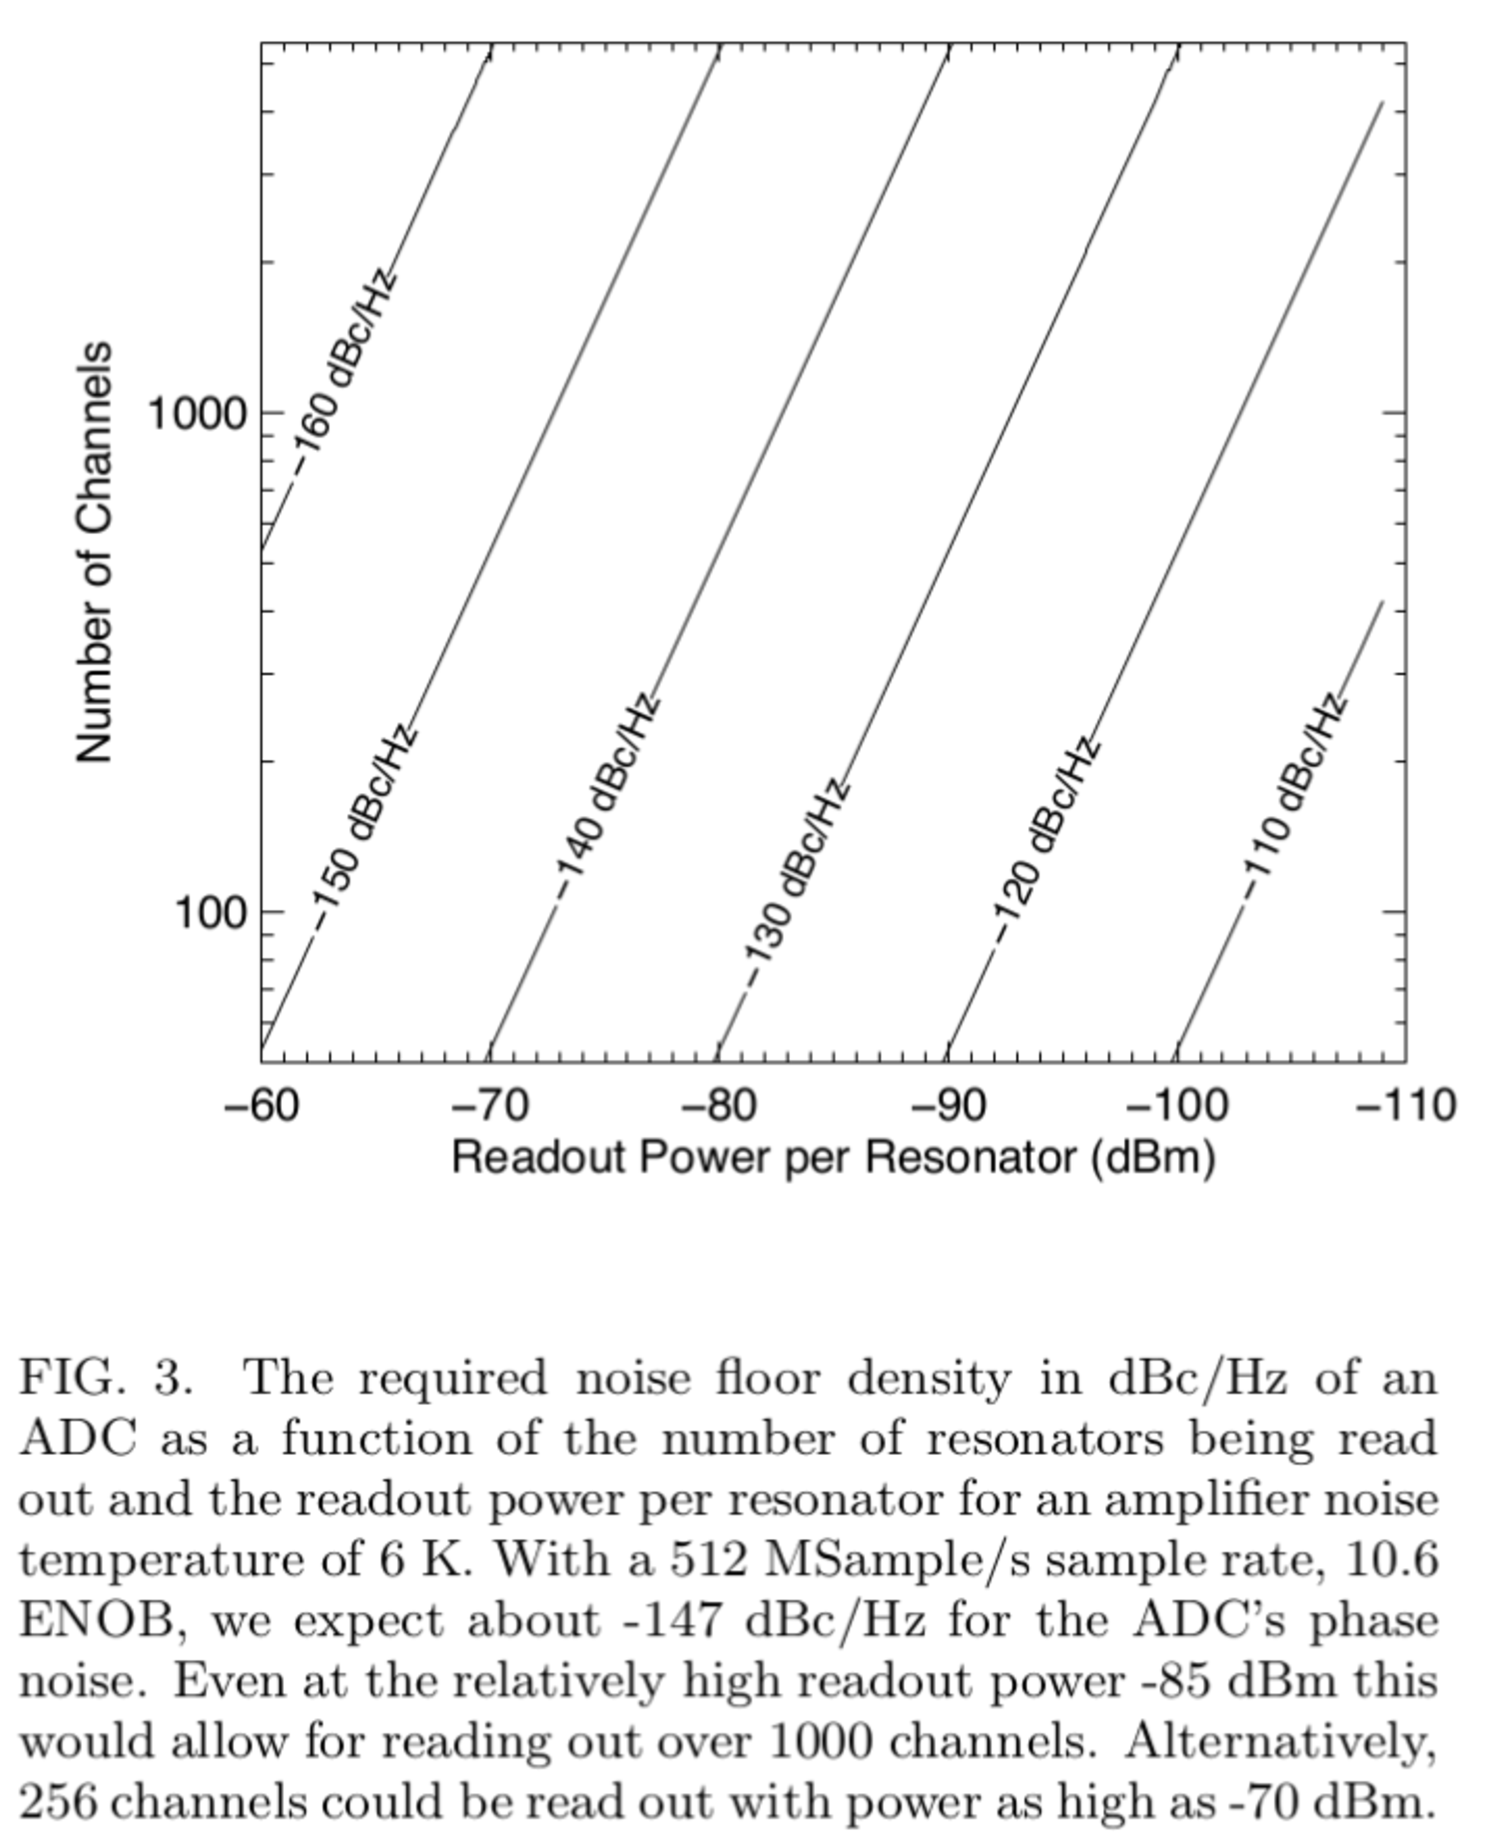
\includegraphics[width=0.85\textwidth]{power_vs_Nchannels}
								\end{column}
				\end{columns}
\end{frame}

\section{Equipamiento BT}
Using section and subsection commands, outside of frames, provides a table of contents and progress information to beamer.
\begin{frame}{Equipos BT}
				\begin{columns}
								\begin{column}{0.45\textwidth}
												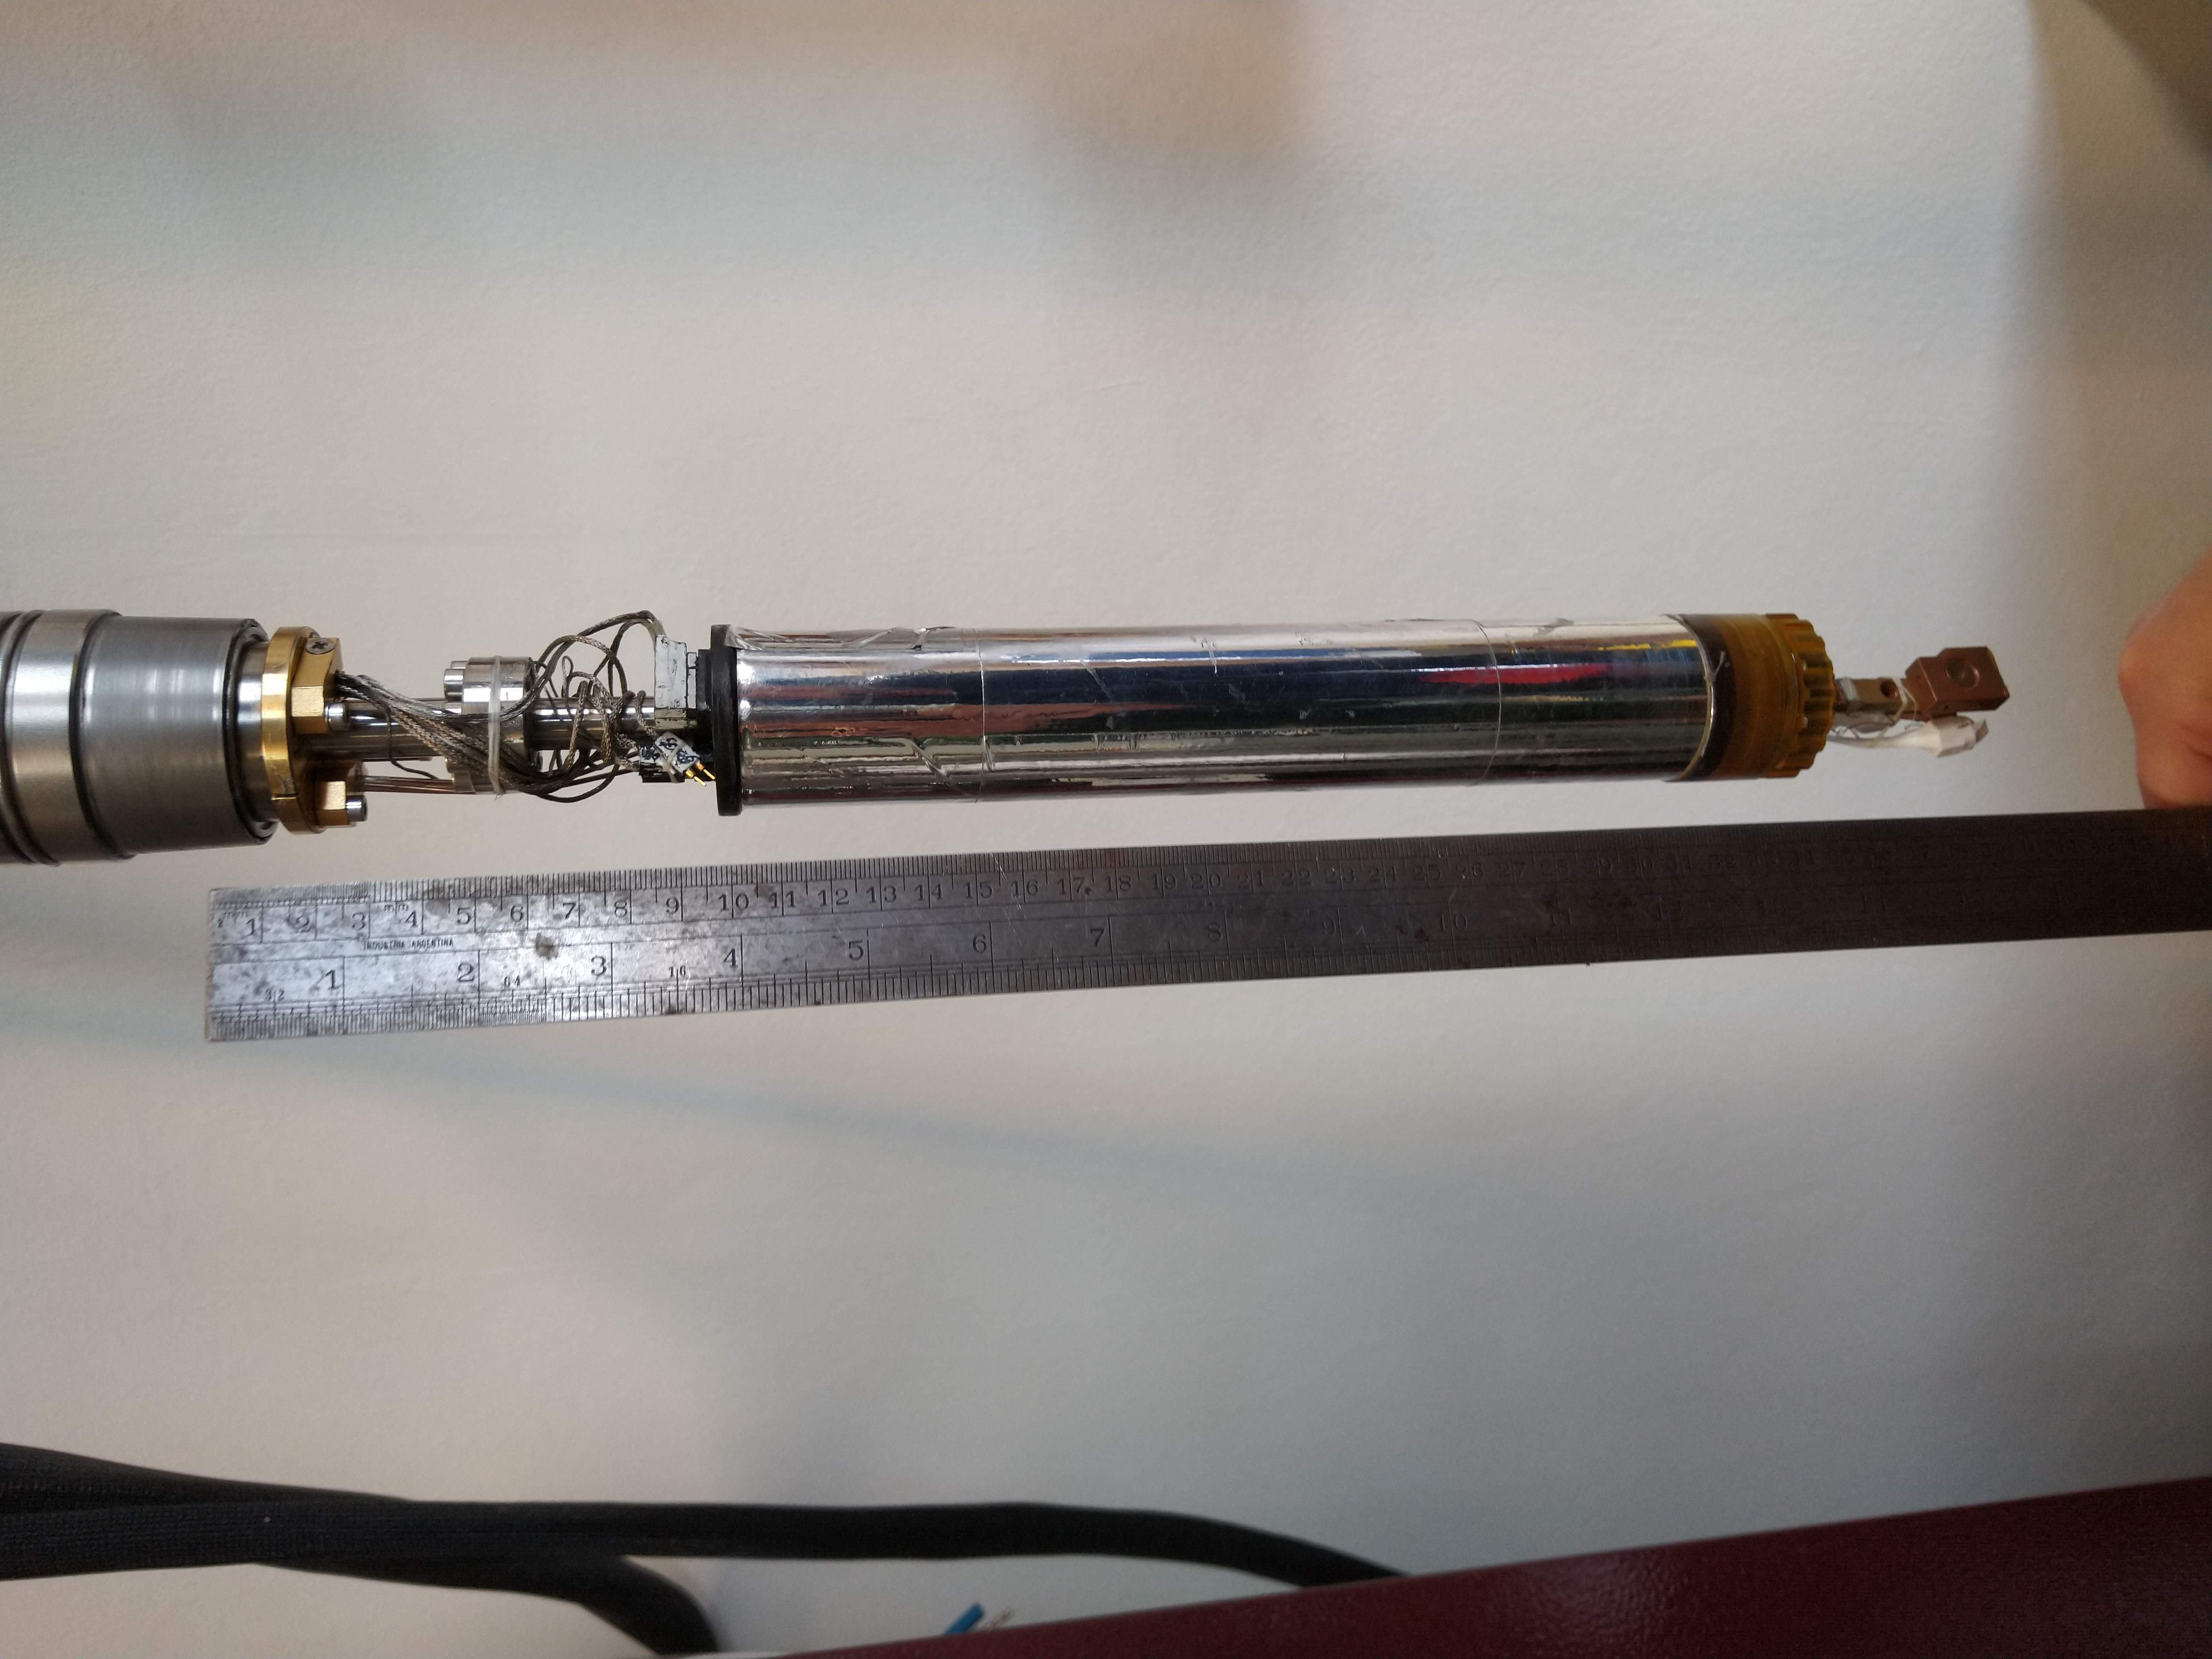
\includegraphics[angle=-90,width=0.62\textwidth]{IMG_20190523_105037648} \\ 
												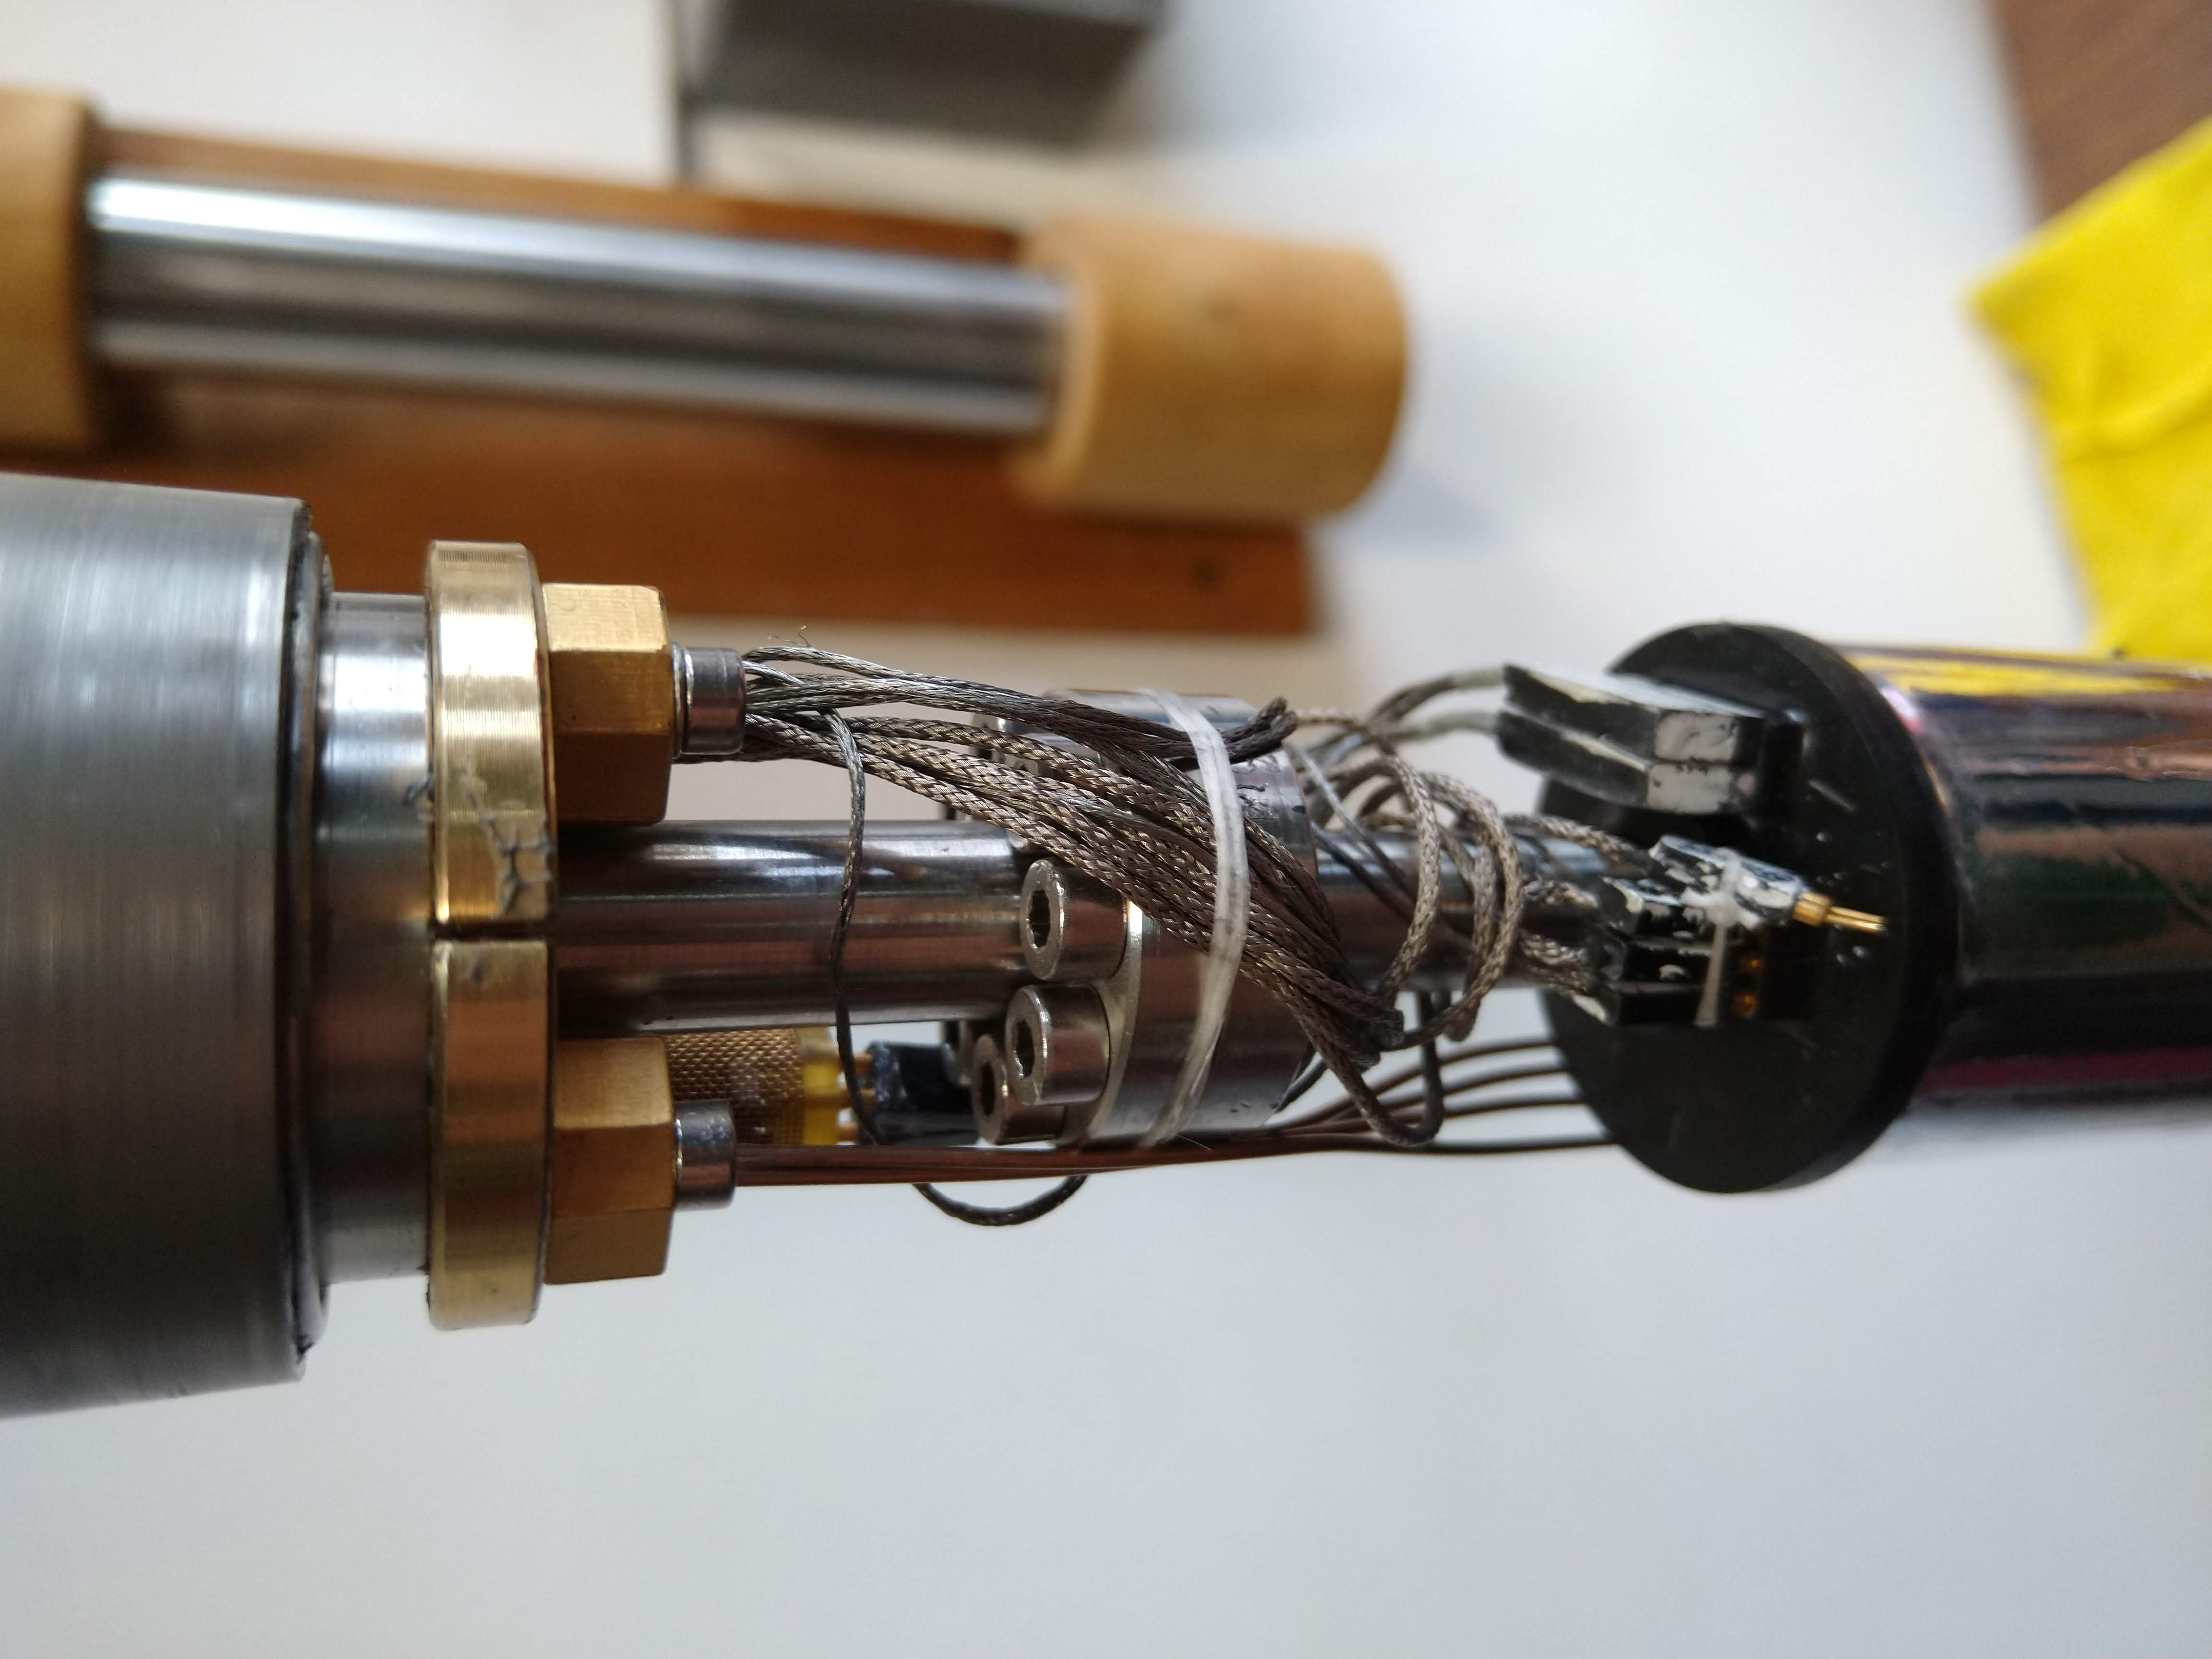
\includegraphics[angle=-90,width=0.6\textwidth]{IMG_20190523_105054061}
								\end{column}
								\begin{column}{0.45\textwidth}
												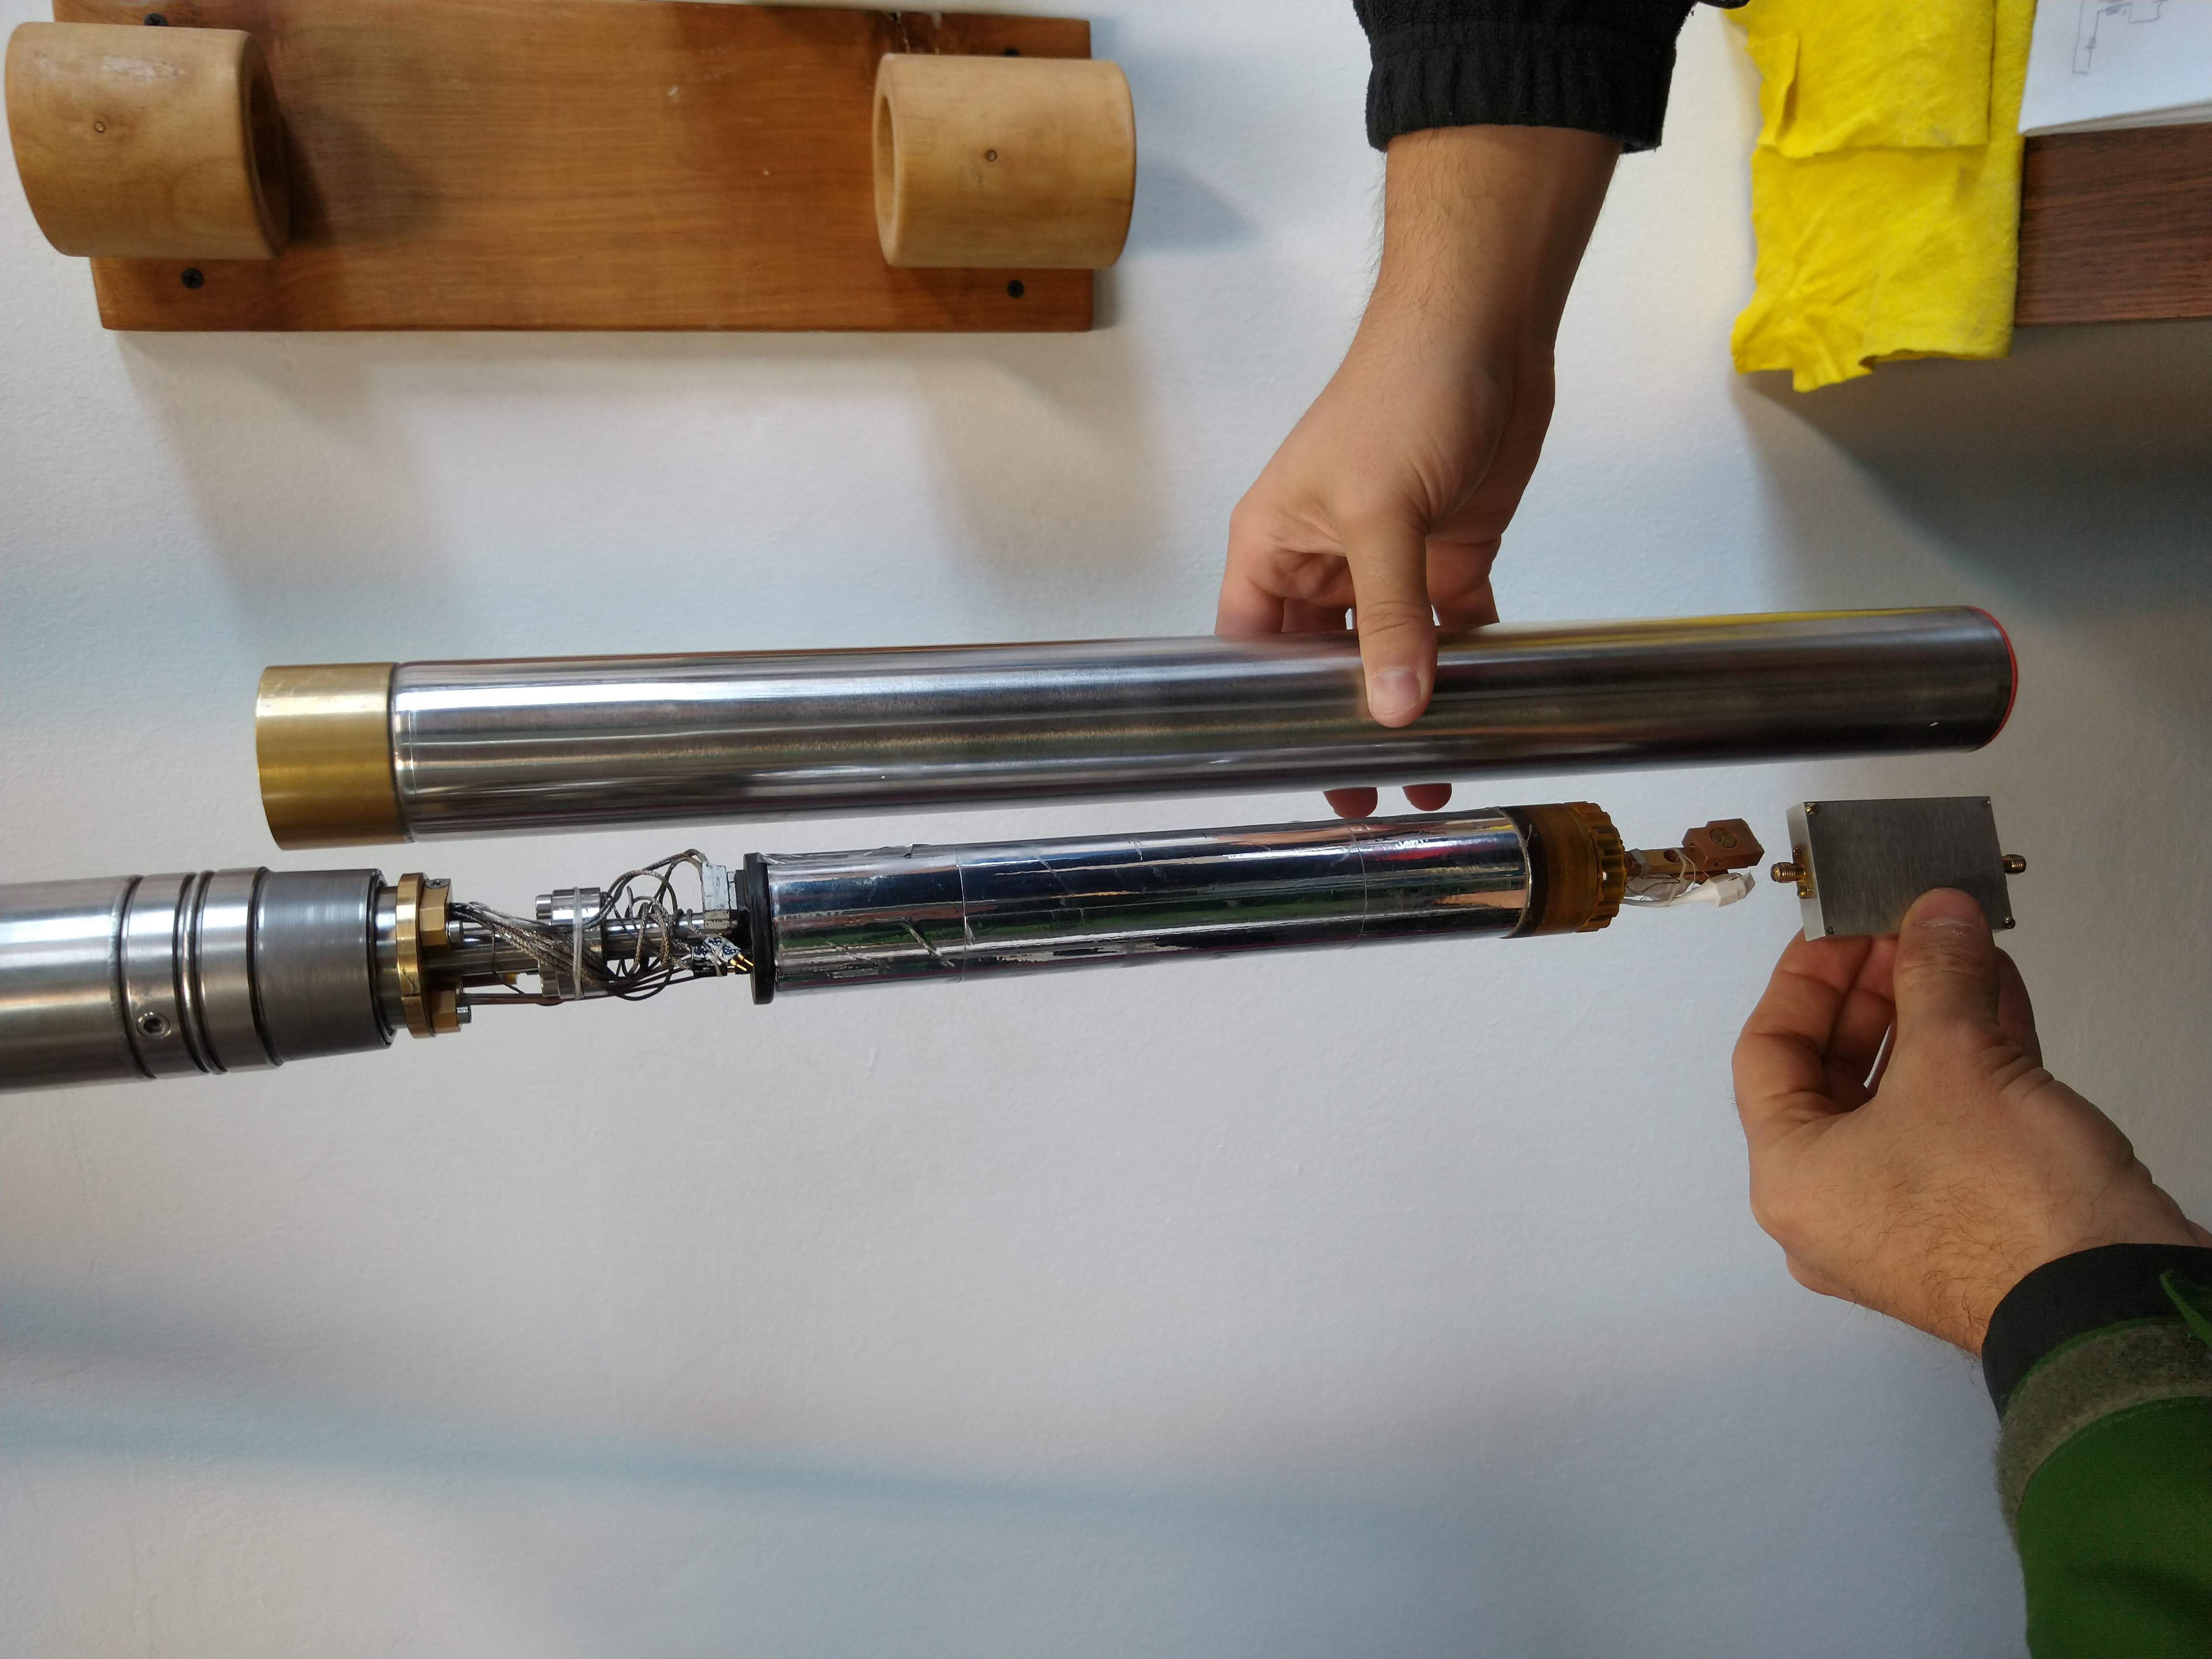
\includegraphics[angle=-90, width=0.62\textwidth]{IMG_20190523_105443289} \\ 
												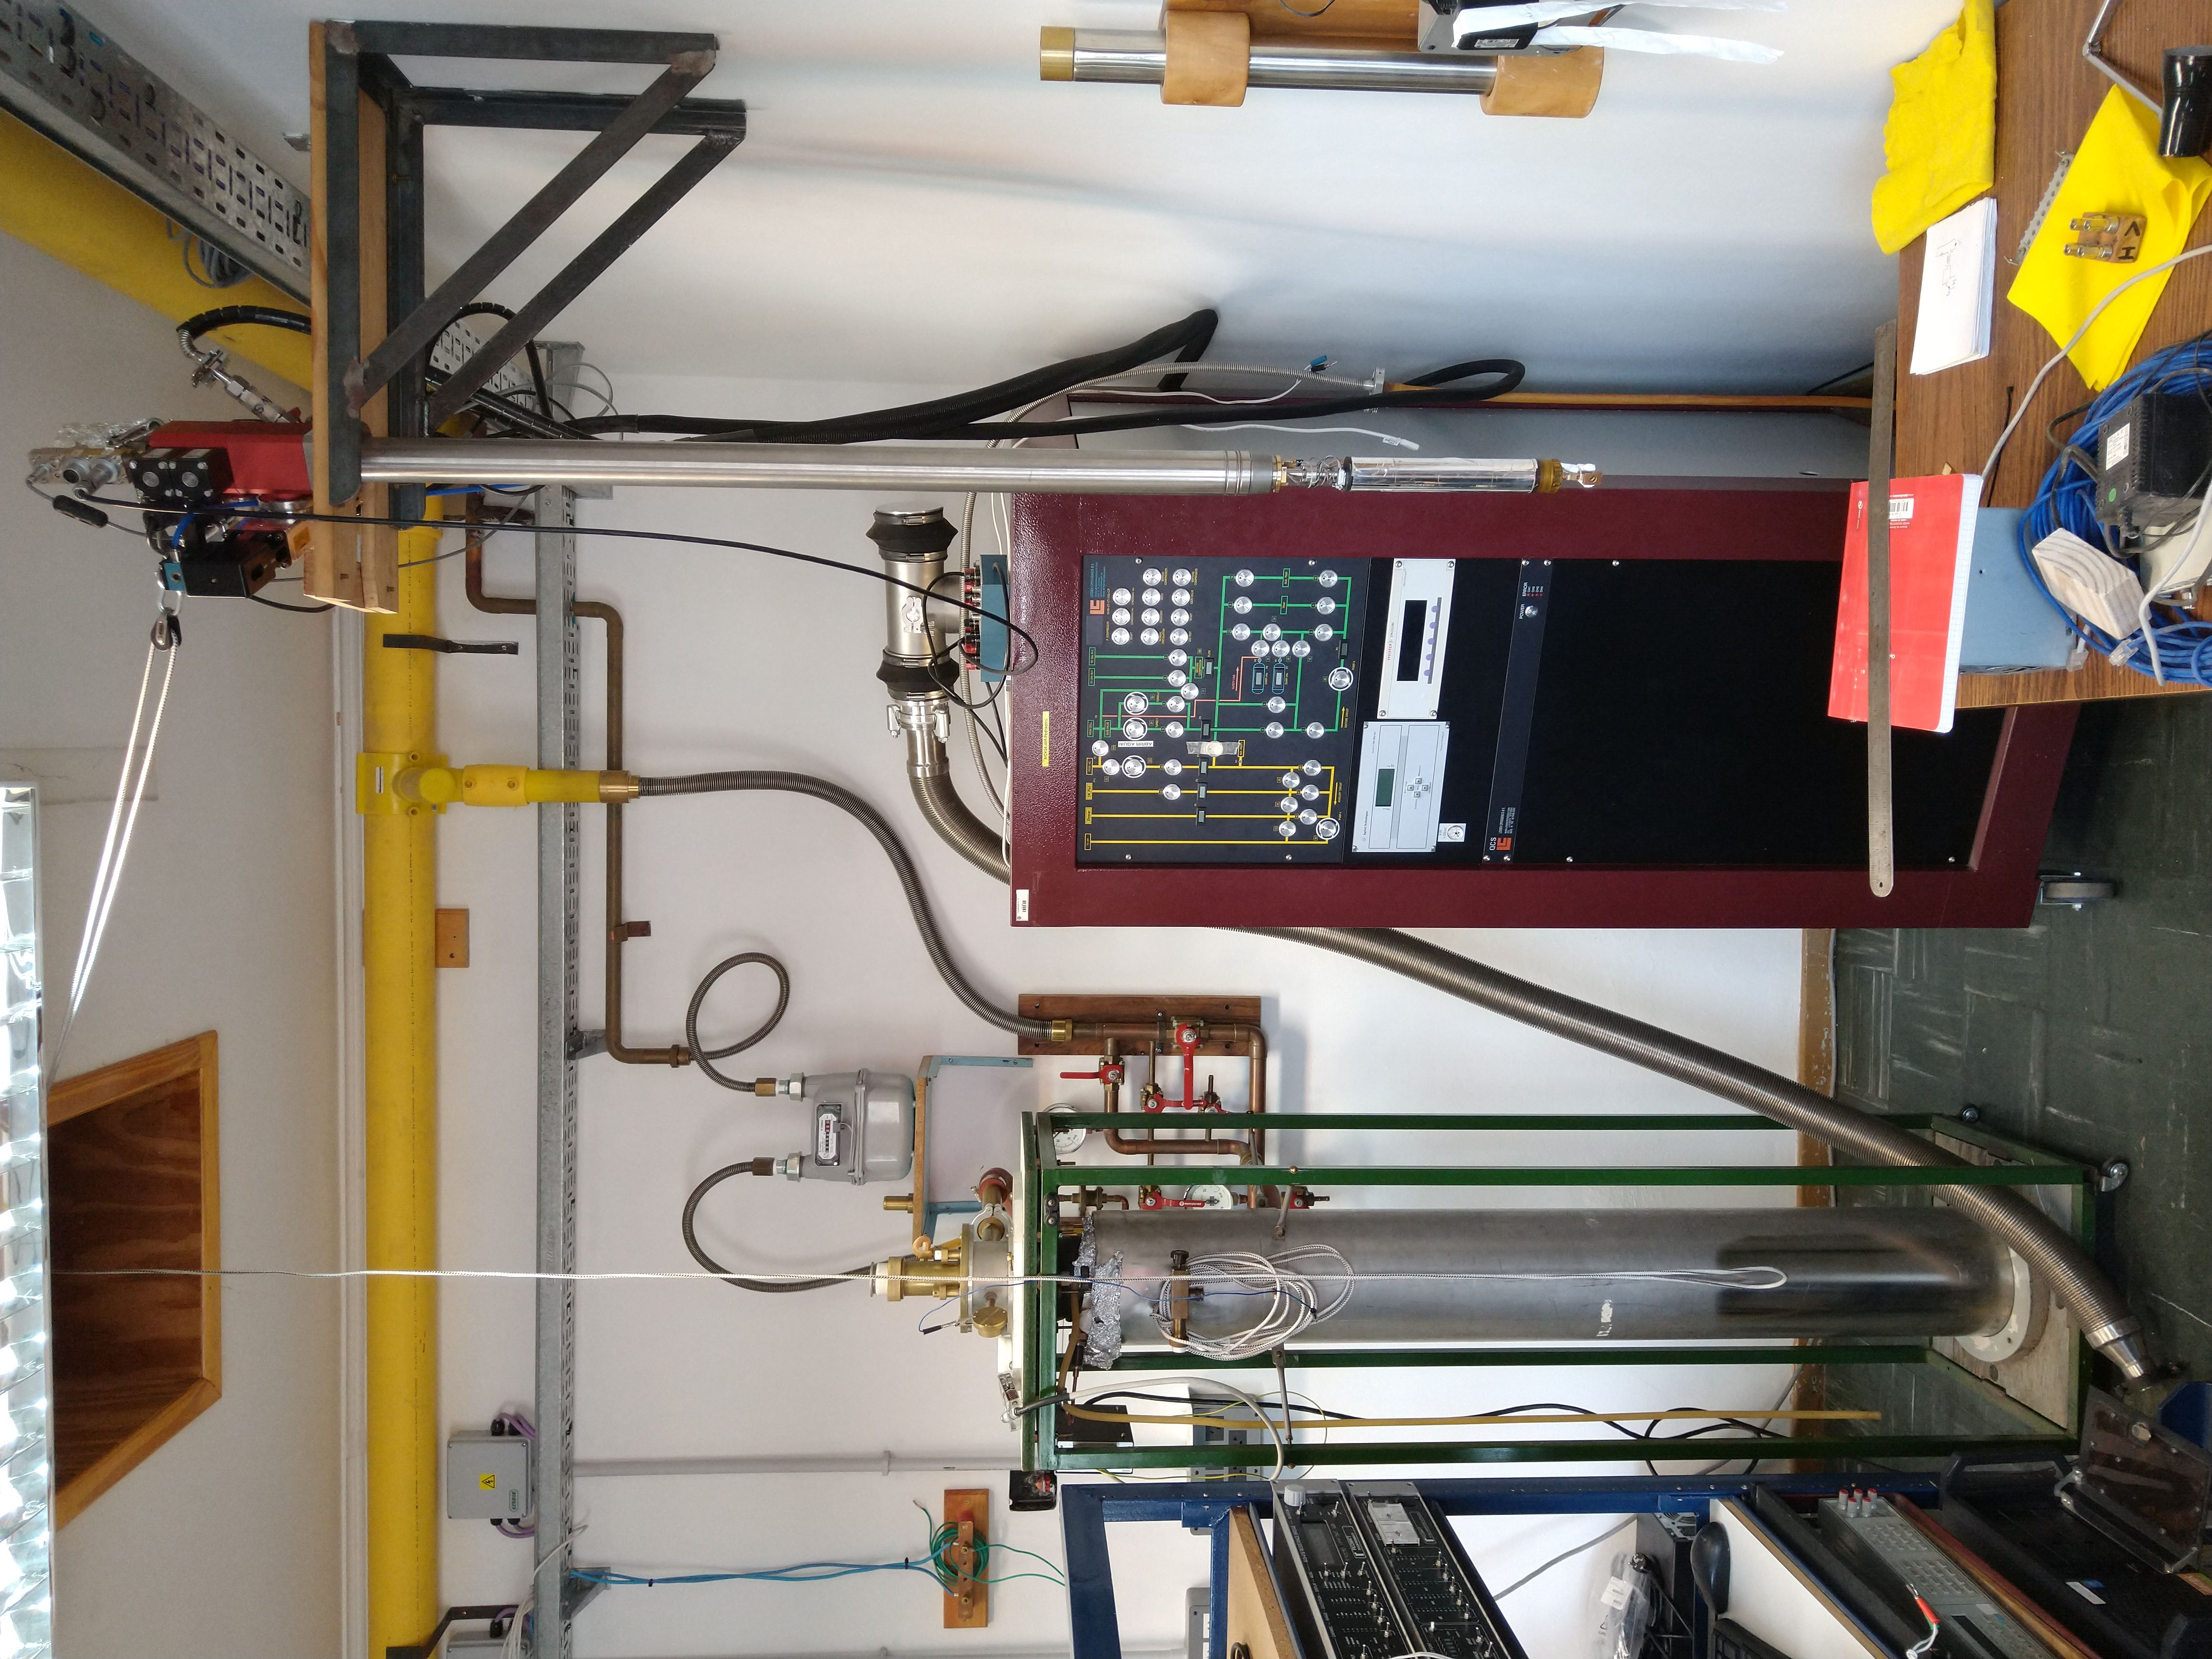
\includegraphics[angle=-90,width=0.6\textwidth]{IMG_20190523_105117465}
								\end{column}
				\end{columns}


				%				Aim for five to ten slides for a 25~minute presentation.
				%
				%				Certainly no more than 15.
				%
				%				Use a note form for the content of each slide.
				%
				%				\begin{theorem}
				%								Mathematics works within the Beamer class, $\exp(i\pi)+1=0$\,, including theorems.
				%				\end{theorem}
				%
				%				Click: \url{http://www.maths.adelaide.edu.au} 
\end{frame}

\begin{frame}{Equipos BT}
				\begin{columns}
								\begin{column}{0.45\textwidth}
												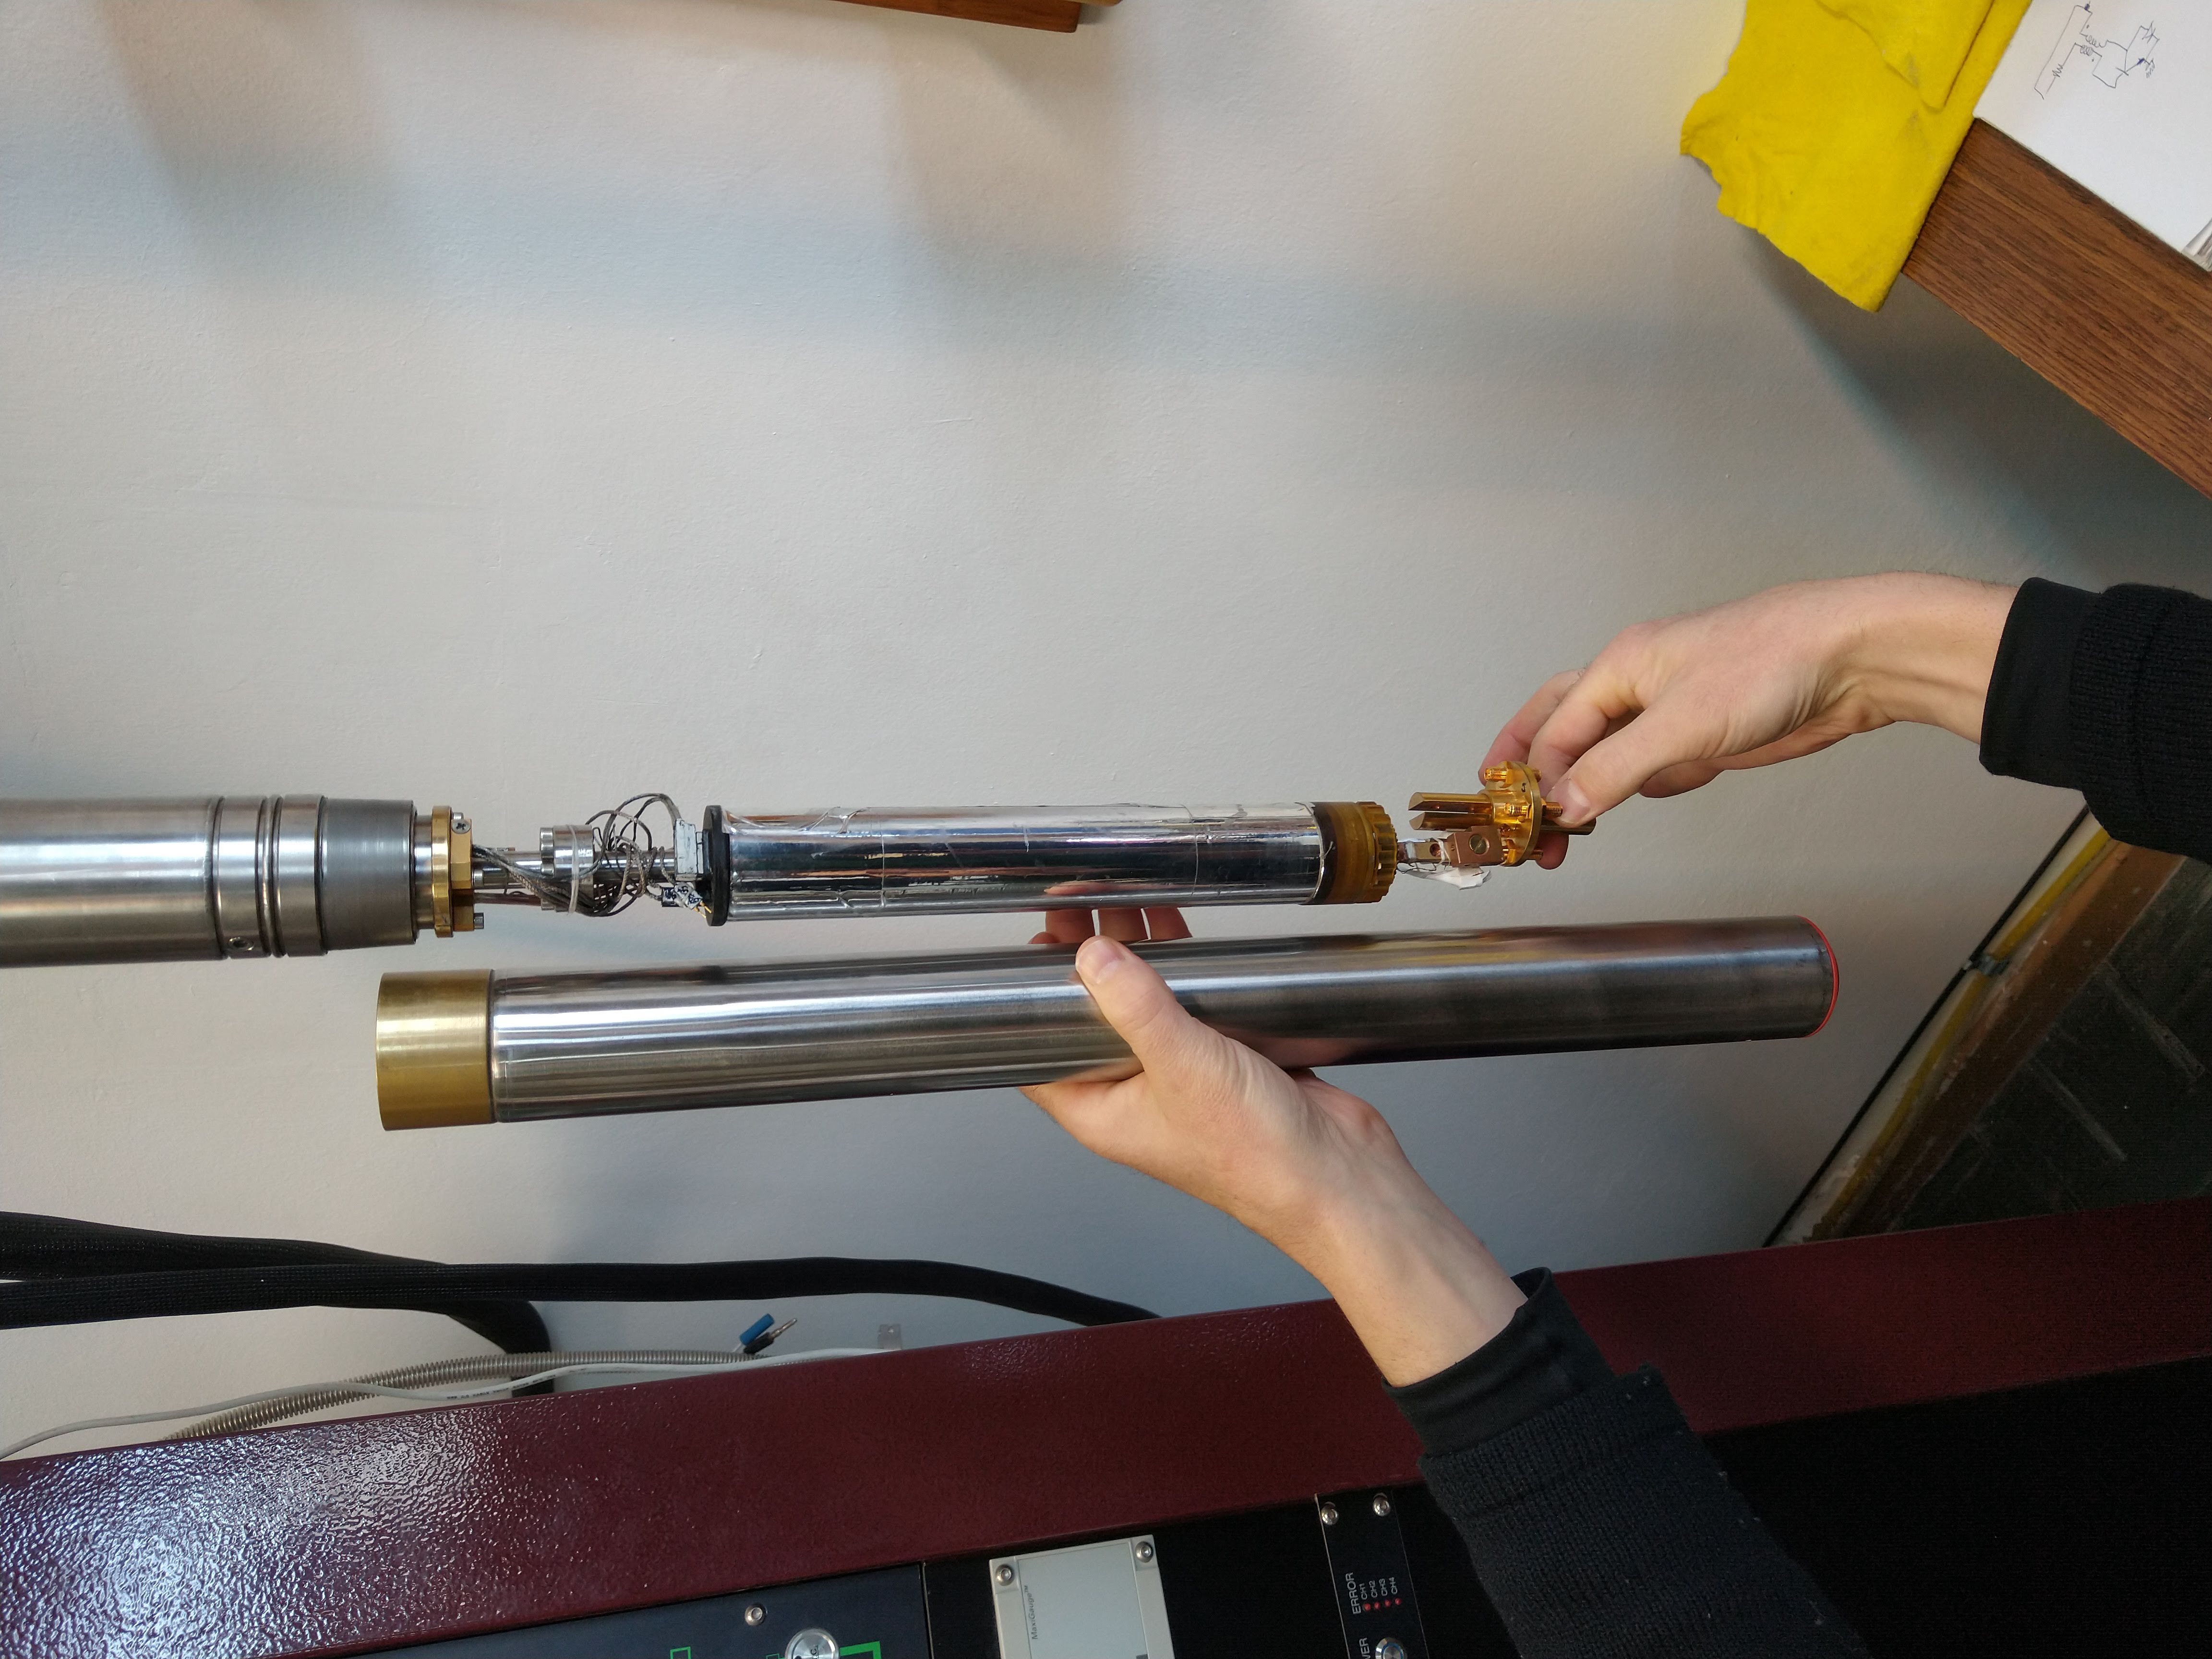
\includegraphics[angle=-90,width=0.62\textwidth]{IMG_20190523_111114131} \\ 
												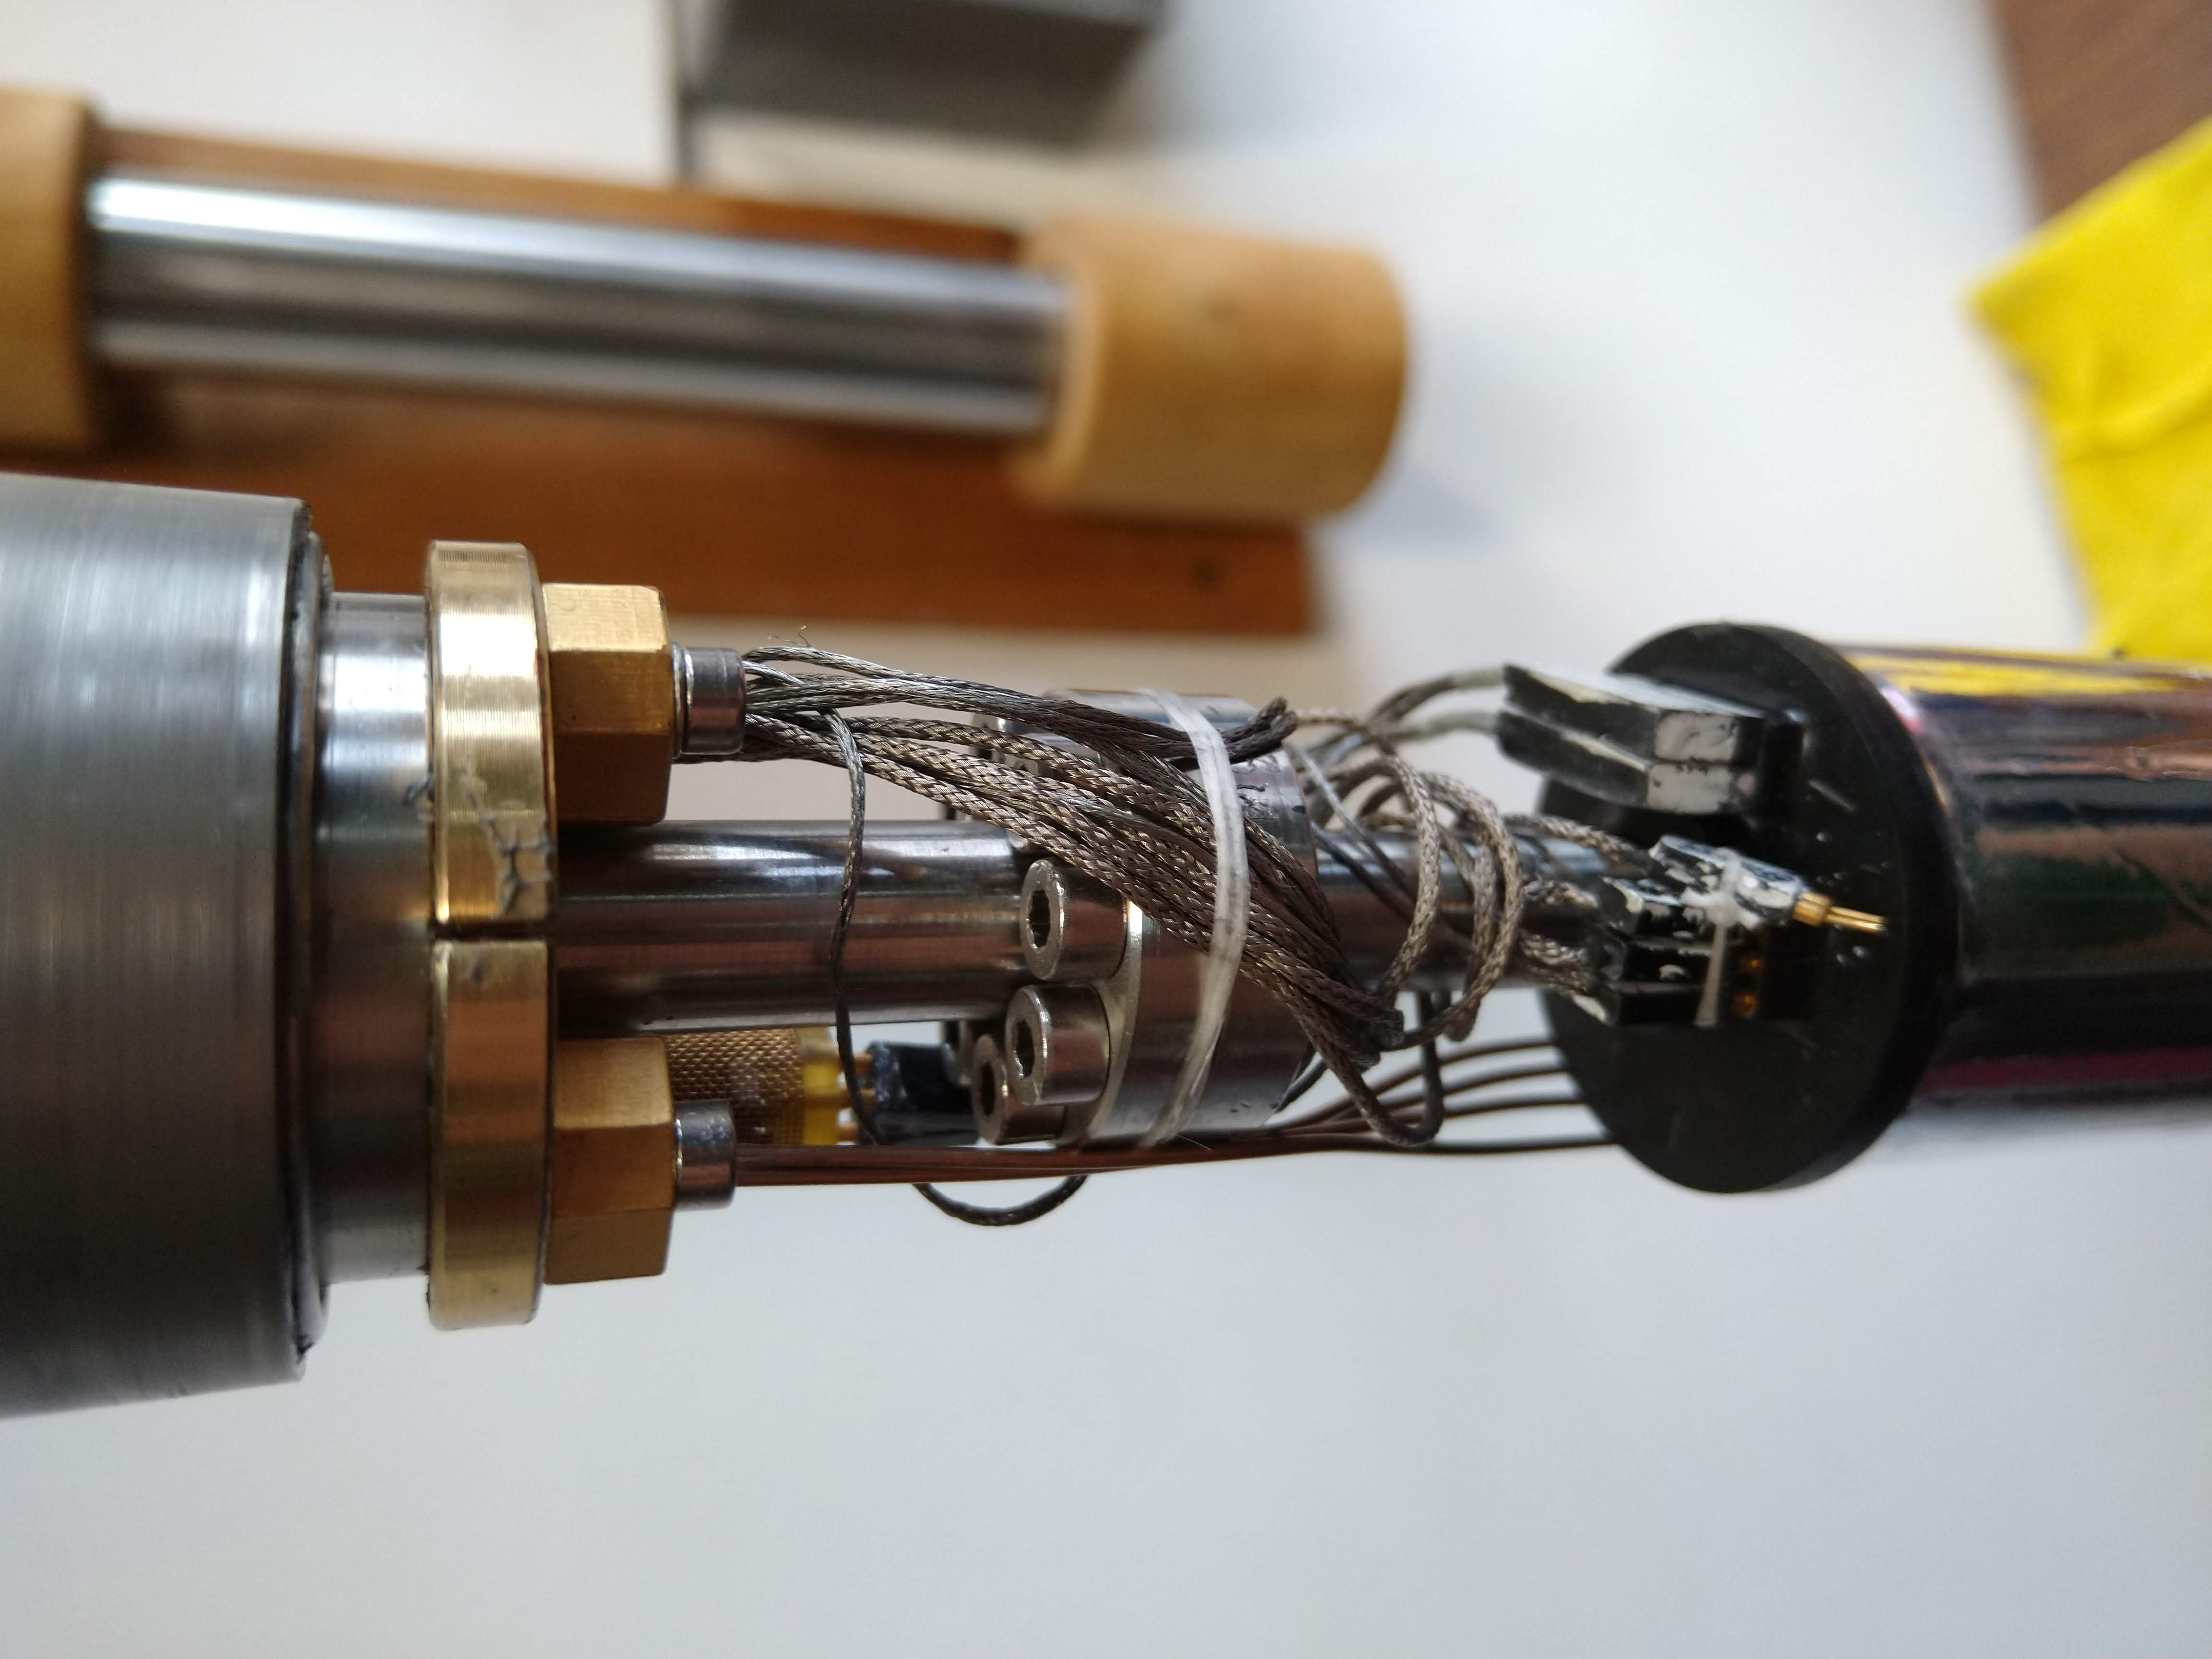
\includegraphics[angle=-90,width=0.6\textwidth]{IMG_20190523_105054061}
								\end{column}
								\begin{column}{0.45\textwidth}
												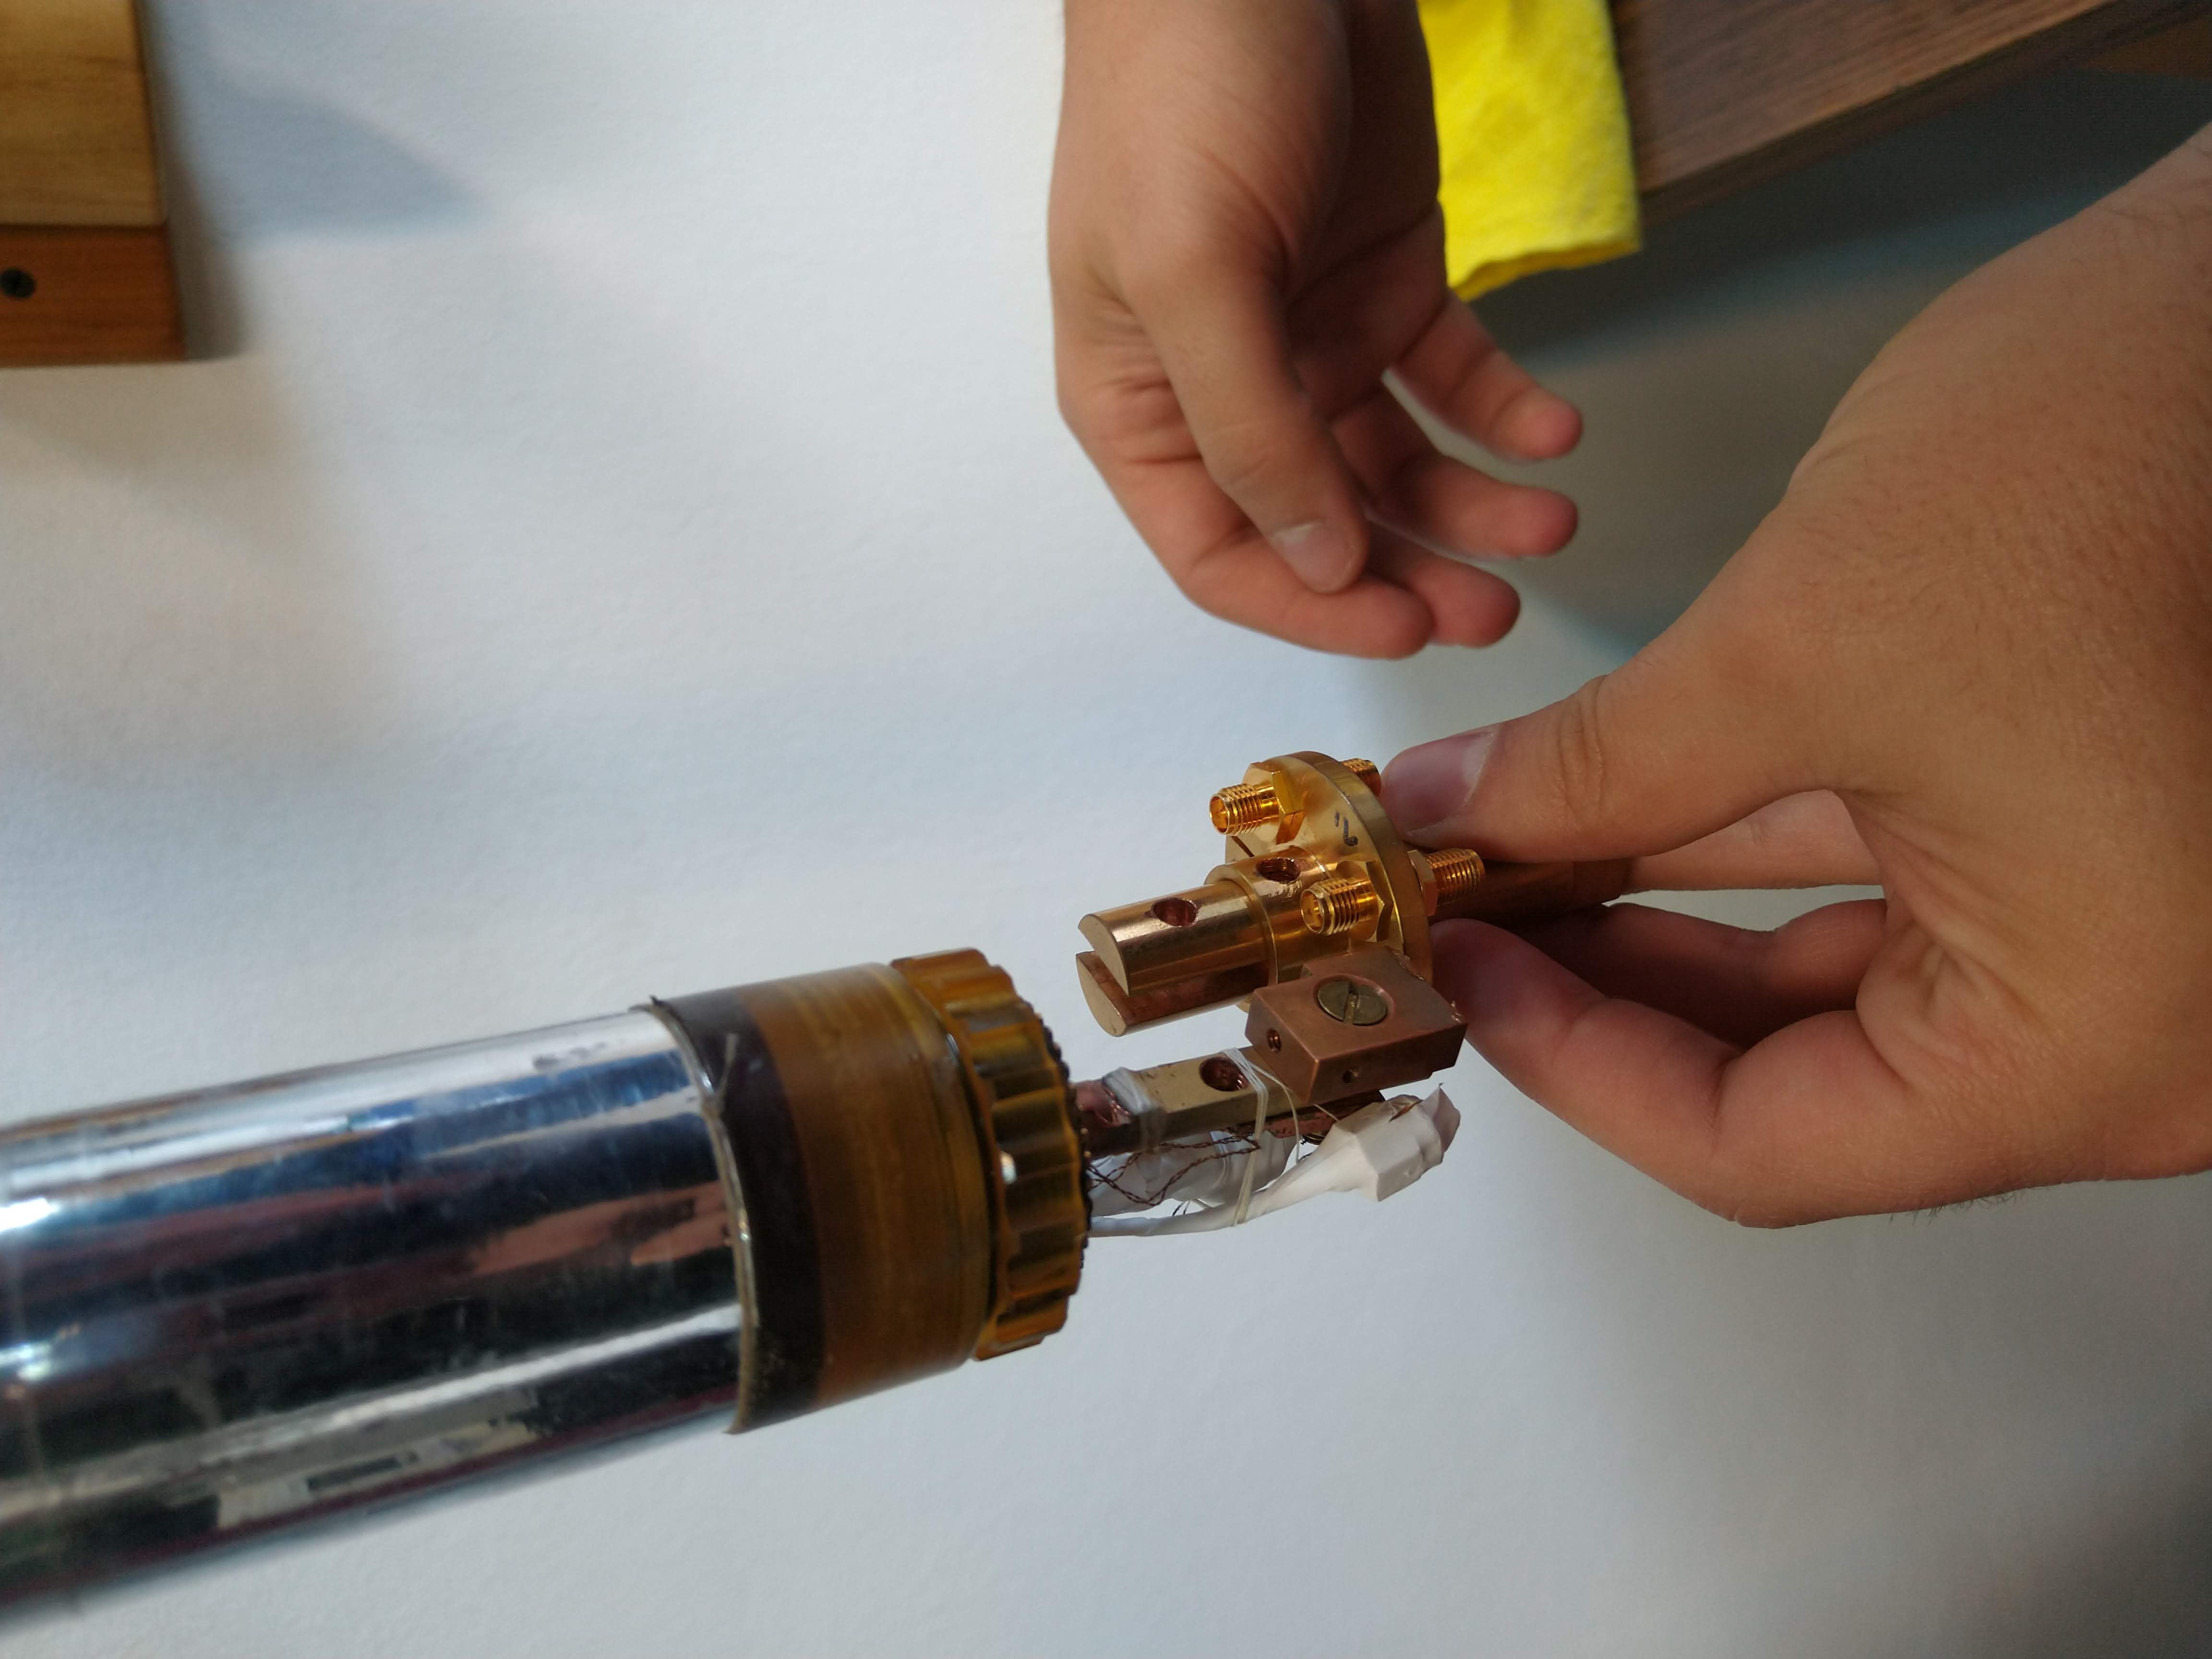
\includegraphics[angle=-90,width=0.42\textwidth]{IMG_20190523_105647049} \\ 
												\hspace{2mm}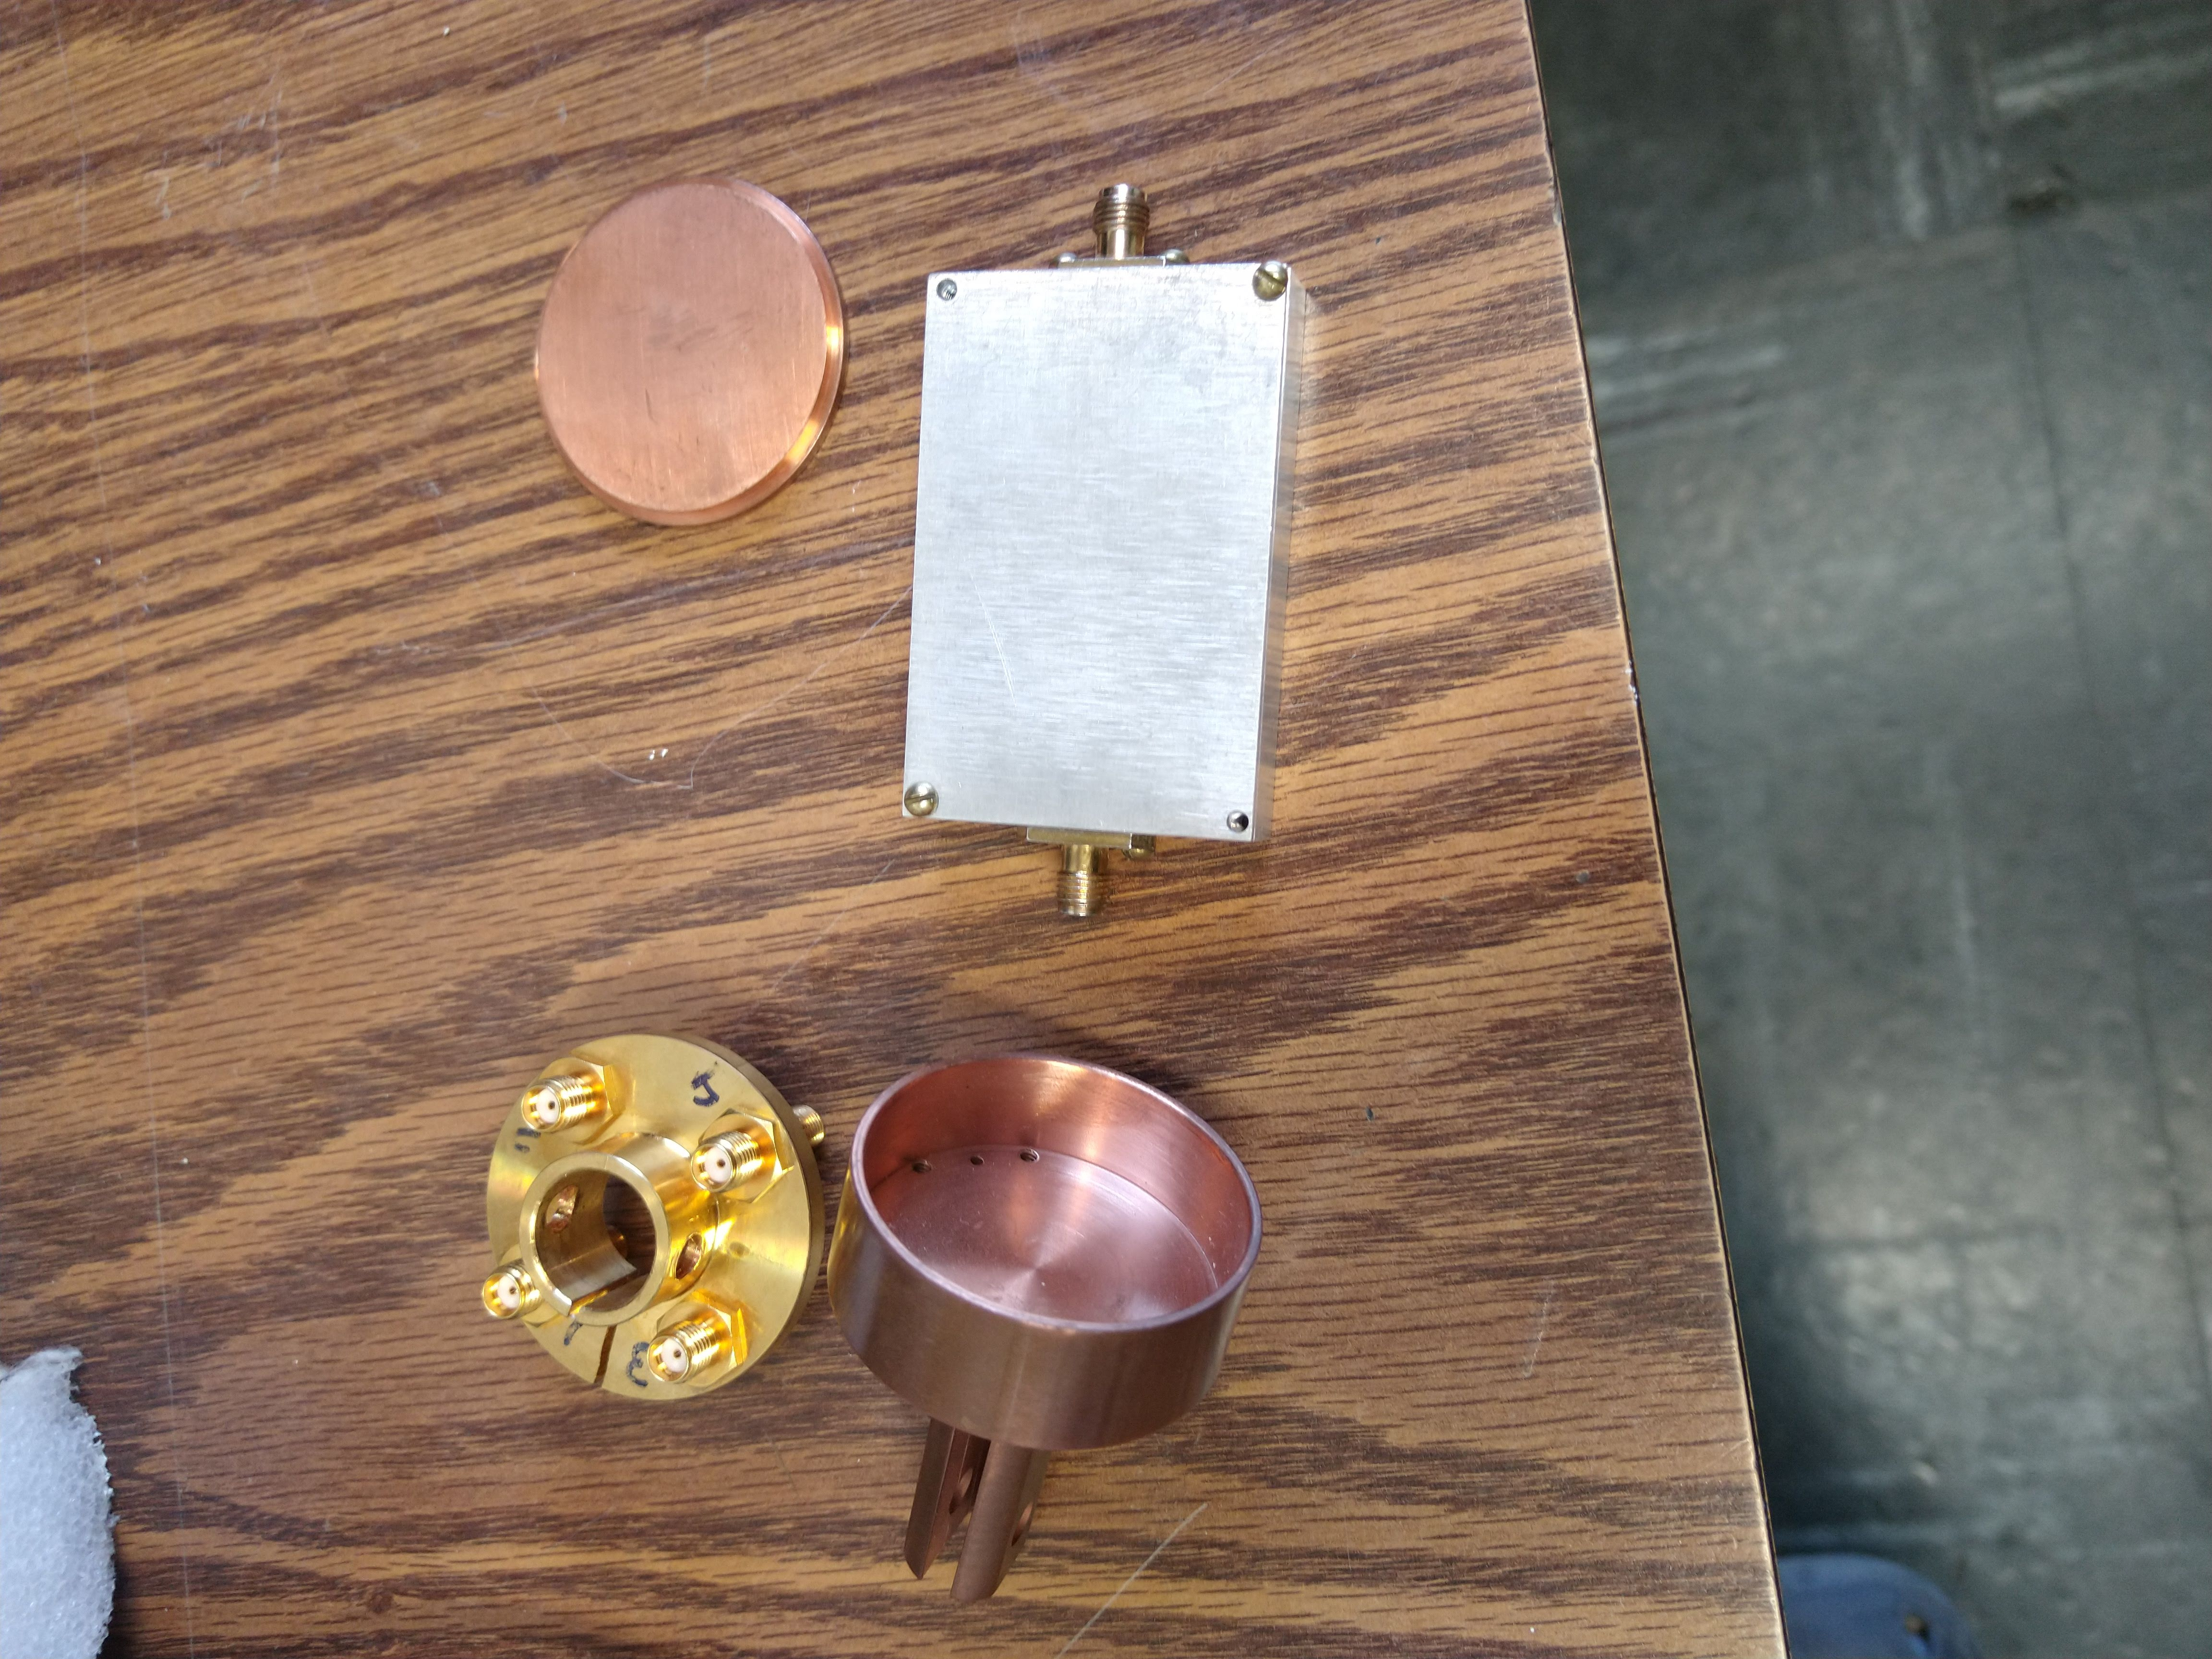
\includegraphics[angle=-90,width=0.42\textwidth]{IMG_20190523_112752228} \\
												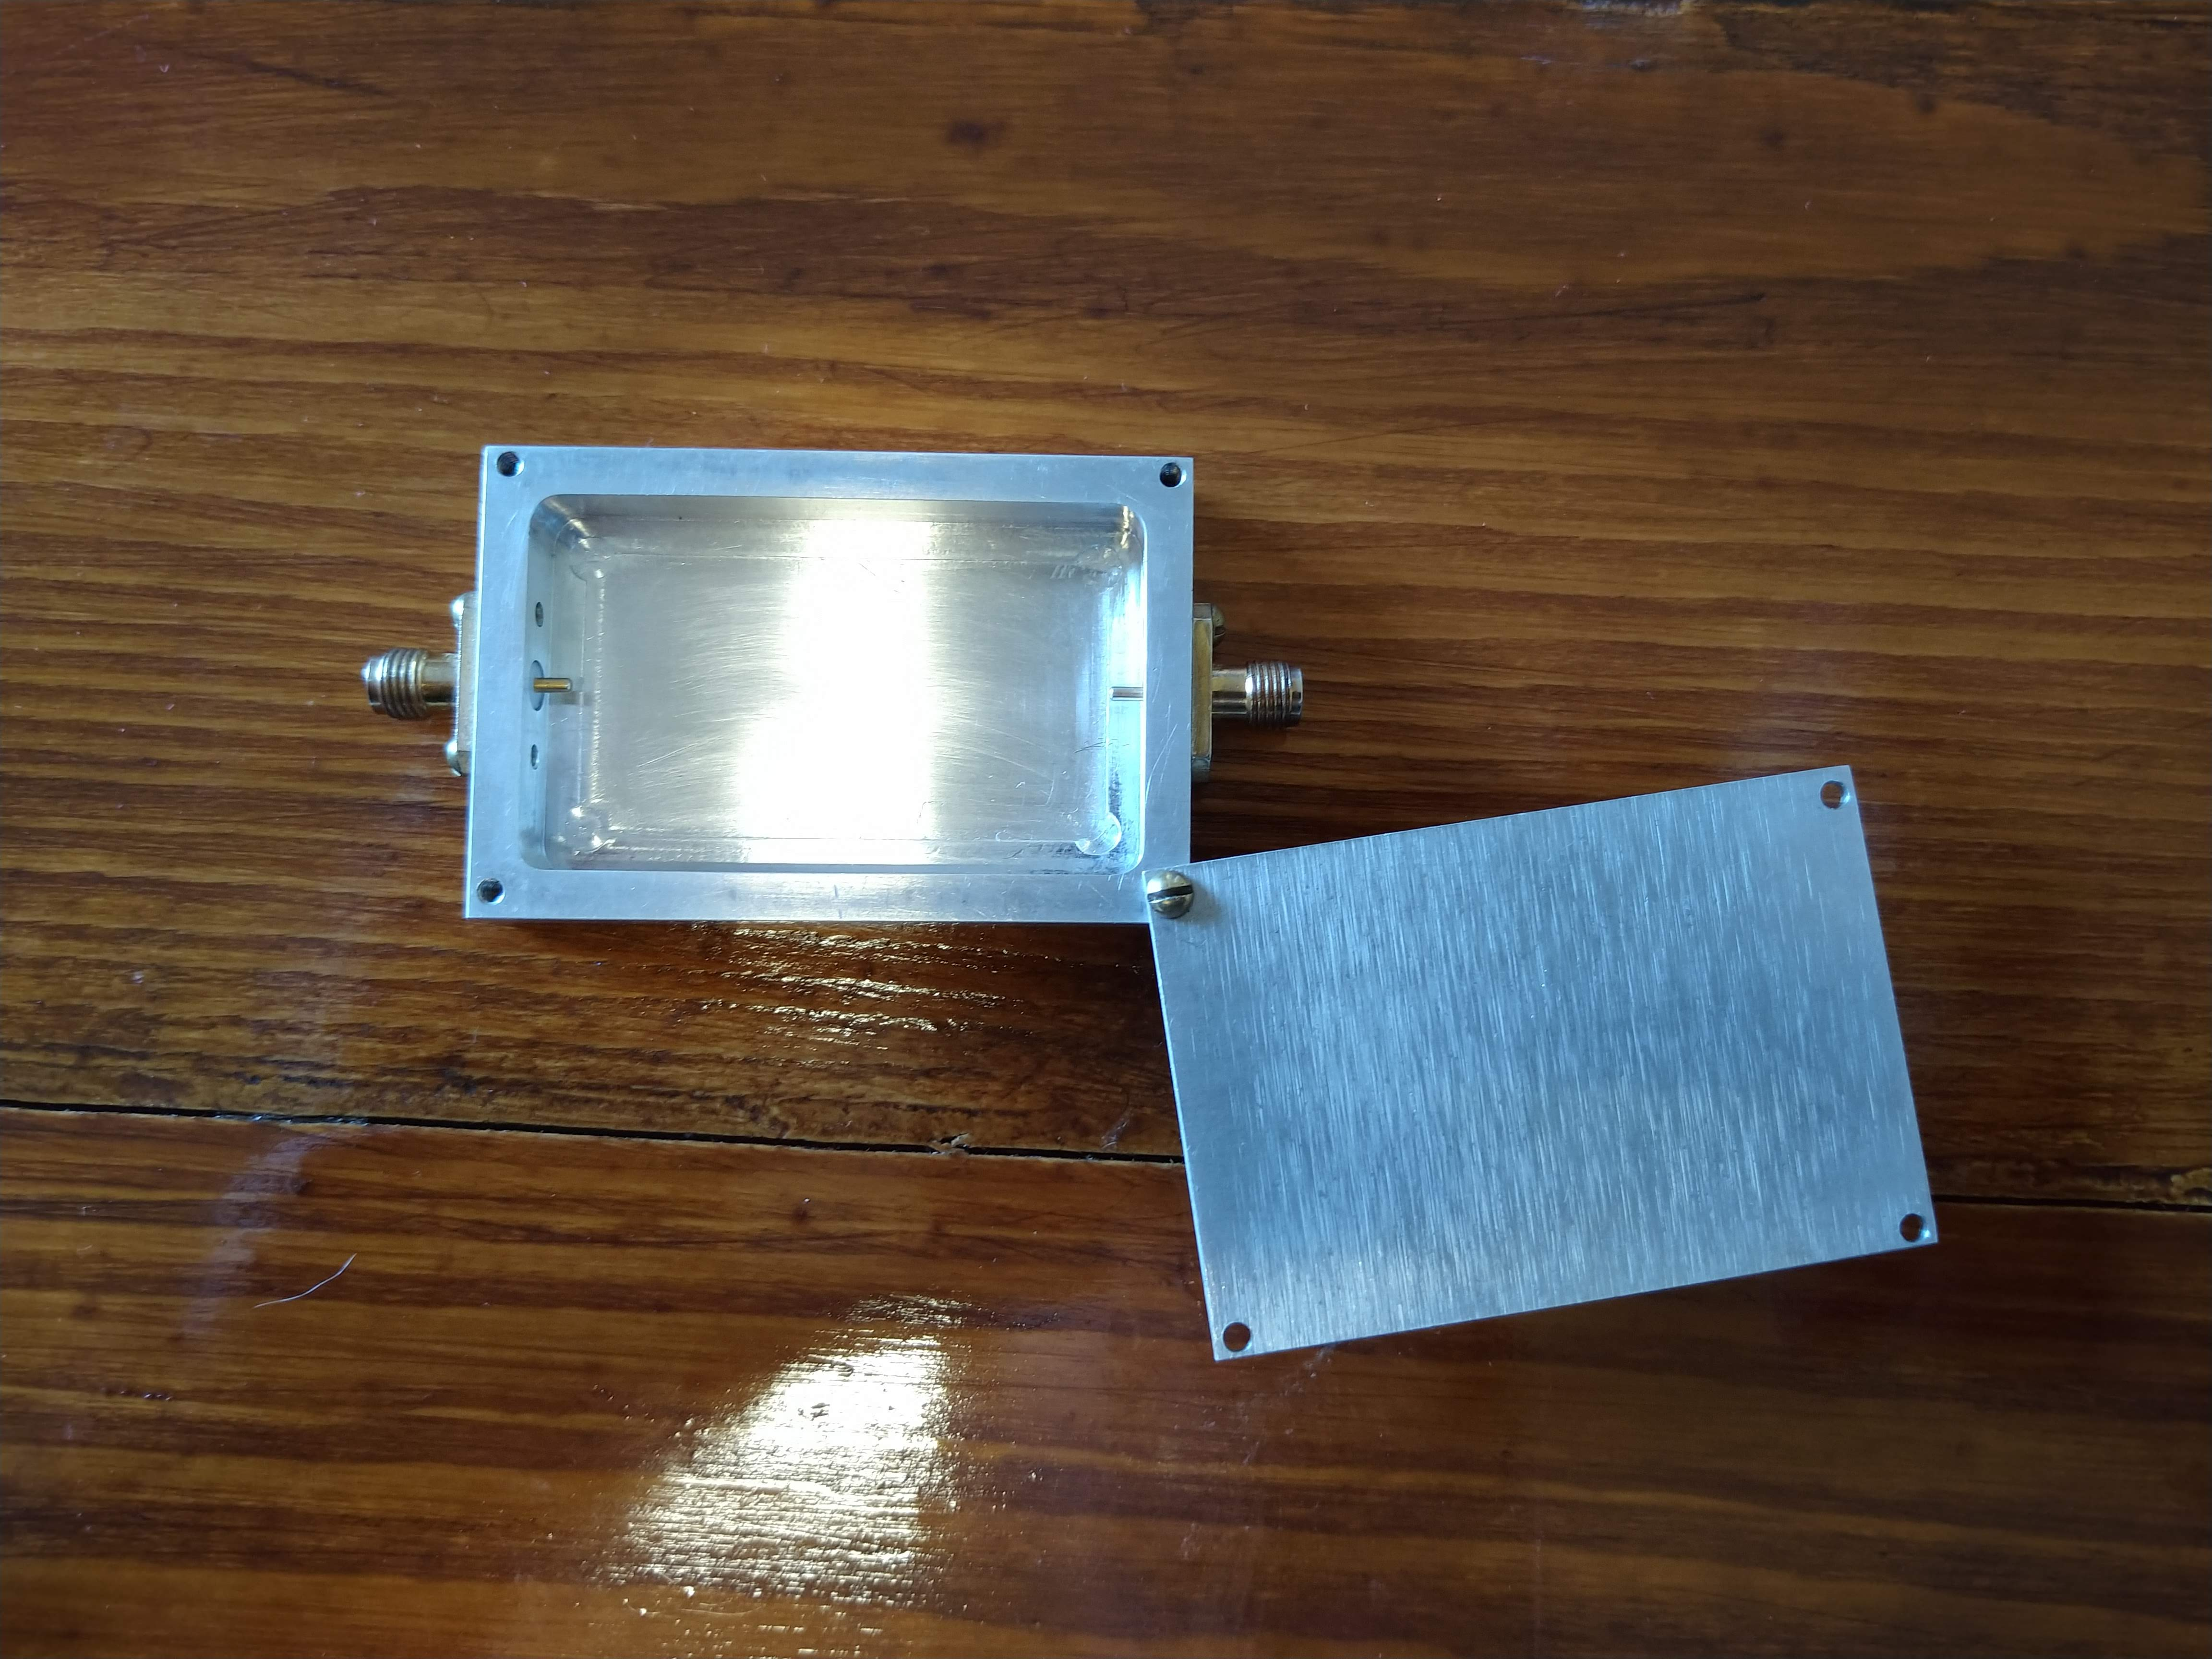
\includegraphics[angle=-90,width=0.42\textwidth]{IMG_20190523_104038976}
								\end{column}
				\end{columns}
				%				Aim for five to ten slides for a 25~minute presentation.
				%
				%				Certainly no more than 15.
				%
				%				Use a note form for the content of each slide.
				%
				%				\begin{theorem}
				%								Mathematics works within the Beamer class, $\exp(i\pi)+1=0$\,, including theorems.
				%				\end{theorem}
				%
				%				Click: \url{http://www.maths.adelaide.edu.au} 
\end{frame}

				\begin{frame}{Amplificador criog\'enico de bajo ruido}
								\framesubtitle{LNF-LNC03\_14A}
								\begin{columns}
												\begin{column}{0.40\textwidth}
																\hspace{10mm}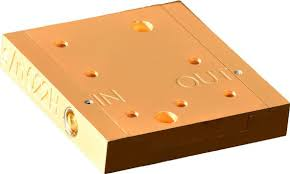
\includegraphics[width=0.95\textwidth]{lnf-lnc03_14sa}
												\end{column}
												\begin{column}{0.60\textwidth}
																\begin{itemize}
																				\item Ancho de Banda RF: 0.3-14 GHz
																				\item Ruido: 4.1 K (típico)
																				\item Ganancia: 42 dB
																				\item Potencia DC: Vc= 0.7 V @ 14 mA
																				\item Conectores RF: G3PO Macho
																				\item Conector DC: Nano Strip 5 pines hembra
																\end{itemize}
												\end{column}
								\end{columns}
				\end{frame}



\section{Perspectivas de trabajo}
\begin{frame}{Perspectivas de trabajo}
				\begin{itemize}
								\item Dise\~no de resonador en Sonnet
								\item Primeras mediciones a $T_{amb}$ y $T \sim 100\,mK$
								\item Definici\'on de requerimientos para crio (cables,
												conectores, espacios, etc.)
								\item Primeras pruebas con RxChannelizer con ITeDA (pruebas de
												front-end, mezcladores, filtros, DC-block, etc.)
				\end{itemize}
\end{frame}
%\section{Prefer titles that make a statement}
%\begin{frame}{Prefer titles that make a statement}
%
%				Many opt for meaningless titles and section titles.  
%
%				Instead, make titles convey information.
%
%				\pause
%
%				Use \texttt{pause} commands almost anywhere to progressively step through material.
%
%				\pause
%
%				\begin{figure}
%								\centering
%								\caption{Figure and table environments also work.
%								Use \texttt{includegraphics} or \texttt{pgfplots}.}
%								\begin{tikzpicture}
%												\begin{axis}[footnotesize,axis lines=middle
%																,xlabel={$t$},no marks,thick,domain=0:2.2,smooth ]
%																\addplot+[]{1-2*exp(-2*x)+exp(-4*x)};
%																\addlegendentry{$u(t)$};
%																\addplot+[]{1-exp(-4*x)};
%																\addlegendentry{$v(t)$};
%																\addplot+[]{1+2*exp(-2*x)+exp(-4*x)};
%																\addlegendentry{$w(t)$};
%												\end{axis}
%								\end{tikzpicture}
%				\end{figure}
%
%\end{frame}
%
%
%
%
%\section{Conclusion}
%\begin{frame}{Conclusion}
%
%				Finish with your conclusions displayed: \emph{not} a list of references, \emph{nor} a meaningless ``thank you'' slide.
%
%				\vfill
%				\begin{quote}
%								Three rules of public speaking: Be forthright.  Be brief.  Be
%								seated. \hfill(S. Dressel \& J. Chew, 1987)
%				\end{quote}
%\end{frame}




\end{document}

